% ============================================================
% main.tex — Pattern di coordinamento in un social network AI-native
% Tesi di Laurea Triennale — Informatica per la Comunicazione Digitale
% Università degli Studi di Milano
%
% NOTE DI CONVERSIONE (Markdown -> LaTeX), da leggere prima di editare:
%
% 1. NUMERAZIONE FIGURE/TABELLE: nel Markdown originale le tabelle erano
%    numerate per capitolo (Tabella 3.1, 4.1, 5.1, 6.1) ma le figure erano
%    numerate in sequenza globale (Figura 1...9). Qui ho standardizzato
%    ENTRAMBE su numerazione per capitolo (\counterwithin), piu' comune
%    in una tesi e piu' facile da mantenere capitolo per capitolo. Se non
%    va bene, è la riga "\counterwithin{figure}{chapter}" qui sotto da
%    rimuovere.
% 2. INDICE: l'elenco manuale con le stime di pagina (es. "3-4 p.") e'
%    stato sostituito da \tableofcontents, che si genera da solo. Le
%    stime di pagina erano materiale di pianificazione, non contenuto
%    da stampare nella tesi finale.
% 3. CITAZIONI: i riferimenti nel testo (es. "Holtz (arXiv:2602.10131)")
%    sono stati convertiti in \citet{}/\citep{} collegati a references.bib.
%    Vedi quel file per le correzioni fatte sulle singole entry.
% 4. CORREZIONE PRINCIPALE: "Pacheco \& Nizzoli" non esiste come paper
%    congiunto - sono due paper distinti nello stesso volume ICWSM 2021.
%    Corretto in tutto il testo a \citet{pacheco2021} (solo Pacheco et al.).
%    Vedi nota dettagliata in references.bib.
% 5. Sezioni con %TODO indicano punti che richiedono una tua decisione o
%    verifica, non semplici refusi di conversione.
% ============================================================

\documentclass[12pt,a4paper]{report}

% --- Codifica, lingua, font ---
\usepackage[utf8]{inputenc}
\usepackage[T1]{fontenc}
\usepackage[italian]{babel}

% --- Layout ---
\usepackage[a4paper,margin=2.8cm]{geometry}
\usepackage{setspace}
\onehalfspacing

% --- Matematica ---
\usepackage{amsmath}
\usepackage{amssymb}

% --- Tabelle, figure, numerazione per capitolo ---
\usepackage{graphicx}
\usepackage{booktabs}
\usepackage{longtable}
\usepackage{array}
\usepackage{float}
\usepackage{caption}
\counterwithin{table}{chapter}
\counterwithin{figure}{chapter}

% --- Bibliografia: natbib, stile autore-anno ---
\usepackage[round,authoryear]{natbib}
\bibliographystyle{plainnat}

% --- Codice / nomi tecnici ---
\usepackage{xcolor}
\newcommand{\code}[1]{\texttt{#1}}
\newcommand{\todonote}[1]{\par\noindent\colorbox{yellow!40}{\parbox{\dimexpr\linewidth-2\fboxsep}{\textbf{TODO:} #1}}\par}

% --- Link e riferimenti incrociati (caricato per ultimo) ---
\usepackage[hidelinks]{hyperref}

\begin{document}

% ============================================================
% FRONTESPIZIO
% ============================================================
\begin{titlepage}
\centering
{\large Università degli Studi di Milano\par}
\vspace{0.3cm}
{\large Corso di Laurea in Informatica per la Comunicazione Digitale\par}
\vspace{2.5cm}
{\Large\bfseries Pattern di coordinamento in un social network AI-native:\\[0.3cm] analisi strutturale e multi-view di Moltbook\par}
\vspace{2.5cm}
{\large Tesi di Laurea Triennale\par}
\vspace{2.5cm}

\begin{flushleft}
\large
\textbf{Relatore:} Prof. Matteo Zignani \\[0.8cm]
\textbf{Candidato:} Riccardo Alliegro
\end{flushleft}

\vfill
{\large Anno Accademico 2025--2026\par}
\end{titlepage}

\tableofcontents
\clearpage

% ============================================================
\chapter{Introduzione}
% ============================================================

\section{Moltbook come caso studio}

Negli ultimi anni, la proliferazione di agenti autonomi basati su modelli linguistici di grandi dimensioni (LLM) ha sollevato interrogativi inediti sulla natura delle interazioni sociali mediate da intelligenza artificiale. Fino a oggi, la ricerca sul comportamento coordinato nei social network si è concentrata quasi esclusivamente su contesti misti, in cui agenti artificiali (bot) coesistono con utenti umani e il problema centrale consiste nel distinguere le due popolazioni. Moltbook introduce uno scenario radicalmente diverso: una piattaforma social popolata esclusivamente da agenti AI, in cui la distinzione umano-bot non è più pertinente ma in cui emergono nuove domande sul coordinamento e sull'organizzazione spontanea del comportamento collettivo.

Moltbook è stato lanciato il 28 gennaio 2026 da Matt Schlicht e Ben Parr. In poche settimane ha raggiunto milioni di agenti registrati, attirando l'attenzione della comunità scientifica e del settore tecnologico. Il 10 marzo 2026 la piattaforma è stata acquisita da Meta, che ha integrato il team fondatore nei propri laboratori di ricerca sull'intelligenza artificiale. La disponibilità di un'API pubblica senza autenticazione ha reso Moltbook un caso di studio eccezionalmente accessibile per la ricerca accademica.

Il presente lavoro nasce dall'osservazione che, in un contesto AI-native, le tecniche classiche di bot detection basate su segnali semantici e lessicali perdono efficacia: tutti gli agenti producono testo generato da LLM, rendendo i detector stilometrici e i classificatori AI-vs-human sostanzialmente non informativi. Questo collasso del segnale semantico sposta necessariamente l'analisi verso le dimensioni strutturali del grafo conversazionale e i pattern temporali di attività — esattamente il dominio della Social Network Analysis applicata al rilevamento di comportamento coordinato.

\section{Research questions}

La domanda principale che guida questa ricerca è la seguente:

\begin{quote}
\itshape
In una rete sociale popolata esclusivamente da agenti AI, esistono gruppi di agenti che condividono pattern strutturali, temporali e comportamentali sufficientemente simili da suggerire coordinamento, e come si differenziano da agenti che operano indipendentemente?
\end{quote}

A questa domanda principale si articolano tre sotto-domande operative:

\begin{itemize}
  \item \textbf{RQ1:} Qual è la struttura della rete conversazionale di Moltbook e come si confronta con le proprietà attese di social network umani?
  \item \textbf{RQ2:} Costruendo una similarity network multi-view sugli agenti, emergono cluster densi compatibili con ipotesi di coordinamento?
  \item \textbf{RQ3:} I cluster identificati trovano riscontro in metodi indipendenti di anomaly detection, e quali cluster mostrano evidenza convergente di comportamento anomalo?
\end{itemize}

Una nota sul framing linguistico è necessaria fin dall'inizio. La formulazione ``suggerire coordinamento'' e ``compatibili con ipotesi di coordinamento'' è un hedging deliberato e metodologicamente fondato: in assenza di ground truth verificabile, non è possibile affermare l'esistenza di coordinamento intenzionale. Ciò che è possibile identificare sono \emph{firme strutturali} — pattern statisticamente anomali che, in letteratura, sono associati a comportamento coordinato. Questa distinzione sarà mantenuta rigorosa lungo tutto il testo.

\section{Contributo originale}

Il contributo principale di questa tesi si articola su tre livelli.

\textbf{Livello empirico.} È stato costruito da zero un dataset originale attraverso un crawler personalizzato che ha estratto dall'API pubblica di Moltbook 311.448 post, 794.814 commenti e i profili di 27.107 agenti, con copertura temporale dal 28 gennaio al 15 aprile 2026. Il grafo conversazionale risultante comprende 191.671 archi diretti. Questo lavoro costituisce la prima caratterizzazione esclusivamente strutturale del coordinamento su Moltbook, operando interamente su feature comportamentali e topologiche senza ricorso a segnali semantici.

\textbf{Livello metodologico.} La tesi adatta il framework di \citet{pacheco2021} per il rilevamento di Coordinated Inauthentic Behavior (CIB) a un contesto AI-native, in cui il segnale discriminante non può essere semantico. La pipeline proposta opera esclusivamente su feature strutturali, temporali e comportamentali, combinando clustering non supervisionato, anomaly detection e analisi di assortatività in un approccio multi-layer.

\textbf{Livello interpretativo.} I risultati mostrano l'emergenza di cluster con firme comportamentali distinte, due dei quali presentano evidenza convergente da metodi indipendenti — concentrazione anomala nelle top anomalie di IsolationForest e marcato isolamento conversazionale intra-cluster — compatibile con ipotesi di coordinamento.

\section{Struttura della tesi}

Il Capitolo 2 presenta il background teorico e la letteratura correlata su bot detection, CIB e social network AI-native. Il Capitolo 3 descrive il dataset, l'architettura del crawler e la pipeline di feature engineering. I Capitoli 4, 5 e 6 presentano i risultati delle tre research questions. Il Capitolo 7 discute i risultati in relazione alla letteratura e articola le limitazioni metodologiche. Il Capitolo 8 conclude con le implicazioni del lavoro e le direzioni future.

% ============================================================
\chapter{Background e letteratura correlata}
% ============================================================

\section{Coordinated Inauthentic Behavior: framework teorico}

Il concetto di Coordinated Inauthentic Behavior (CIB) è stato formalizzato da Facebook nel 2018 per descrivere reti di account che operano in modo coordinato dissimulando la propria natura e origine. La letteratura accademica ha successivamente operazionalizzato il concetto in termini misurabili.

\citet{pacheco2021} hanno proposto un framework metodologico basato sulla costruzione di una \emph{similarity network} tra account: agenti con profili comportamentali simili vengono collegati, e cluster densi in questa rete vengono identificati come candidati al coordinamento. L'approccio è non supervisionato — non richiede etichette — e si presta naturalmente a contesti in cui il ground truth è assente o non verificabile. Questa tesi adotta e adatta questo framework al contesto AI-native di Moltbook.

La scelta della metrica di coordinamento è centrale nel framework CIB. In letteratura, la coordinazione viene operazionalizzata attraverso la co-attività temporale (account che postano simultaneamente lo stesso contenuto), la co-similarity nei profili di attività, e la struttura topologica delle reti di interazione. Nel nostro caso, la co-activity testuale è esclusa per principio (testo LLM-generated); la coordinazione è quindi misurata attraverso la similarità coseno nello spazio delle feature strutturali e comportamentali.

\section{Bot detection: da lessicale a strutturale}

La ricerca sul rilevamento automatico di bot nei social network ha attraversato tre generazioni metodologiche distinte.

La prima generazione, dominante fino alla metà degli anni 2010, si basava su feature manuali estratte dai profili utente e dai contenuti testuali. Approcci come BotOrNot \citep{varol2017} combinavano centinaia di feature eterogenee — frequenza di posting, rapporto follower/following, presenza di avatar, caratteristiche del testo — in classificatori supervisionati. Questi metodi raggiungevano buone prestazioni su Twitter ma si dimostravano fragili al cambiamento della piattaforma e alle tecniche di evasione.

La seconda generazione ha sfruttato l'informazione di rete, riconoscendo che i bot tendono a formare strutture topologiche peculiari: cluster densi di account mutuamente connessi, pattern di retweeting sincronizzati, rapporti di interazione anomali. \citet{cresci2017} hanno introdotto la nozione di \emph{social spambots} come entità che imitano il comportamento umano a livello individuale ma tradiscono pattern di coordinamento a livello collettivo.

La terza generazione, emergente con la diffusione dei modelli generativi, affronta il problema dell'evasione semantica: un bot alimentato da un LLM può produrre testo indistinguibile da quello umano sia per stile che per contenuto. \citet{cresci2020} e \citet{cresci2025} hanno argomentato che questa evoluzione impone un cambio di paradigma: i segnali discriminanti devono spostarsi dal livello semantico al livello strutturale e comportamentale. Su Moltbook, dove tutti gli agenti producono testo LLM-generated per definizione, i segnali semantici non sono evasivi ma semplicemente non informativi: la dimensione strutturale non è una scelta metodologica alternativa, ma l'unica dimensione pertinente.

\section{Letteratura su Moltbook}

Moltbook ha generato un corpo di ricerca accademica significativo nei mesi successivi al lancio.

\citet{holtz2026} ha condotto la prima analisi strutturale della piattaforma sui dati dei primi 3,5 giorni di vita. I risultati riportati — esponente power-law $\alpha = 1{,}70$, reciprocità 0,197, average path length 2,91 — costituiscono la baseline temporale più prossima al nostro dataset e il riferimento principale per RQ1.

\citet{mukherjee2026}, nel dataset MoltGraph, hanno identificato 5.479 episodi di coordinazione etichettati su dati temporali, offrendo uno dei pochi esempi di ground truth parziale disponibili per questa piattaforma. Il confronto con MoltGraph è identificato come estensione naturale di questo lavoro.

\citet{price2026} hanno documentato i vincoli dell'API pubblica, in particolare il cap di circa 300 commenti distinti per post — un limite metodologico rilevante che questa tesi documenta esplicitamente e quantifica nel Capitolo 3.

\citet{demarzo2026} hanno analizzato un dataset di scala maggiore (369k post, 3 milioni di commenti), offrendo un ulteriore termine di confronto per le statistiche strutturali. MoltNet \citep{moltnet2026} ha analizzato 148k agenti con focus sulla struttura sociale AI-native.

\section{Metodi utilizzati}

\textbf{OddBall} \citep{akoglu2010} è un metodo di anomaly detection strutturale basato sull'analisi delle ego-network. L'osservazione chiave è che, nelle reti reali, esiste una relazione power-law tra il numero di archi dell'ego-network e il numero di triangoli al suo interno. Nodi il cui ego-network si discosta significativamente da questa relazione ricevono un anomaly score elevato. OddBall opera esclusivamente sulla topologia del grafo, indipendentemente dalle feature dei nodi.

\textbf{IsolationForest} \citep{liu2008} è un algoritmo di anomaly detection basato sul principio che i punti anomali sono più facilmente isolabili da alberi decisionali casuali. È applicato alla feature matrix degli agenti come alternativa scalabile a metodi basati su distanza (LOF), particolarmente robusto in alta dimensionalità.

\textbf{Louvain} \citep{blondel2008} è l'algoritmo di community detection adottato sia per la caratterizzazione strutturale del grafo conversazionale (RQ1) sia come validazione alternativa del clustering comportamentale (RQ2). Massimizza la modularity $Q$ in modo greedy gerarchico.

\textbf{Burstiness} \citep{goh2008}: la misura $(\sigma - \mu)/(\sigma + \mu)$ sugli intervalli temporali tra eventi cattura la natura irregolare dell'attività. Valori positivi indicano attività a raffiche (\emph{bursty}), valori negativi attività regolare e periodica.

% ============================================================
\chapter{Dataset e metodologia}
% ============================================================

\section{La piattaforma Moltbook}

Moltbook è una piattaforma di microblogging in cui tutti gli agenti registrati sono sistemi AI. Gli agenti pubblicano post organizzati in \emph{submolt} — comunità tematiche analoghe ai subreddit di Reddit — e interagiscono commentando i post altrui in strutture di thread annidati. La piattaforma distingue tra agenti \emph{claimed} (verificati tramite un account X collegato, attestante una persona reale come proprietaria dell'agente) e agenti \emph{unclaimed} (registrati senza proprietario verificato). Nel dataset raccolto, il 98,6\% degli agenti risulta claimed: lo sbilanciamento estremo rende questa distinzione non analizzabile come variabile di classificazione e viene pertanto esclusa dalla pipeline ML.

L'API pubblica di Moltbook non richiede autenticazione per la lettura dei dati. Il rate limit al momento del crawling era di circa 200 richieste per finestra temporale.

\section{Architettura del crawler}

Il crawler è stato implementato in Python e strutturato in quattro fasi sequenziali, ciascuna con checkpoint di ripresa per garantire la resilienza alle interruzioni.

\textbf{Fase 0} — Raccolta dei metadati di tutti i submolt presenti sulla piattaforma.

\textbf{Fase 1} — Paginazione integrale di tutti i post per ogni submolt. I post sono recuperati in ordine cronologico con pagine da 50 elementi.

\textbf{Fase 2} — Raccolta dei commenti per tutti i post con almeno 3 commenti (\code{MIN\_COMMENTS\_FOR\_CRAWL = 3}). Ogni post viene interrogato tre volte con sort differente (best, new, old) per massimizzare il numero di commenti unici recuperati. La soglia di 3 commenti è stata preferita alla soglia 1--2 perché post con pochi commenti tendono a essere eliminati o vuoti, generando errori HTTP 500.

\textbf{Fase 3/4} — Recupero dei profili di tutti gli agenti scoperti come autori di post o commenti.

Il database di destinazione è SQLite con schema a 5 tabelle: \code{agents}, \code{posts}, \code{comments}, \code{submolts}, \code{agent\_features}. Tutte le operazioni di lettura e scrittura sono centralizzate nel modulo \code{db.py}.

Gli archi del grafo conversazionale sono derivati dal campo \code{parent\_id} dei commenti: se l'agente A risponde al commento dell'agente B, viene registrato un arco diretto A $\rightarrow$ B. Questo meccanismo di inferenza degli archi dalla struttura dei thread è l'unica modalità disponibile, poiché l'API pubblica non espone endpoint per follower o following.

\section{Dataset raccolto}

La raccolta dati è stata condotta tra il 28 gennaio e il 15 aprile 2026. Il dataset finale è riportato in Tabella~\ref{tab:dataset-stats}.

\begin{table}[H]
\centering
\caption{Statistiche del dataset.}
\label{tab:dataset-stats}
\begin{tabular}{@{}lr@{}}
\toprule
Metrica & Valore \\
\midrule
Agenti totali & 27.107 \\
Post totali & 311.448 \\
Commenti totali & 794.814 \\
Archi conversazionali (senza self-loop) & 191.671 \\
Self-loop rimossi & 3.585 (1,9\% degli archi) \\
Agenti claimed & 26.738 (98,6\%) \\
Copertura temporale & 28 gen -- 15 apr 2026 \\
\bottomrule
\end{tabular}
\end{table}

\section{Limite strutturale dell'API}

Il vincolo di $\sim$300 commenti distinti per post (3 sort $\times$ $\sim$100) rappresenta un limite metodologico dichiarato. Per i post con numero di commenti superiore a 300 — presumibilmente i post virali — una frazione degli archi conversazionali non è stata catturata. Questo introduce una sottorappresentazione sistematica delle interazioni sui contenuti più popolari, e potenzialmente degli archi degli hub. Il dataset presentato rappresenta la copertura massima ottenibile dall'API pubblica senza autenticazione, dopo paginazione integrale di tutti i submolt e triplo crawling per sort dei commenti.

\section{Subset analitico}

Le analisi di rete (RQ1--RQ3) sono condotte sul sottoinsieme di agenti effettivamente presenti nel grafo conversazionale, definito come gli agenti con almeno un arco in ingresso dopo la rimozione dei self-loop. Il subset comprende \textbf{9.096 agenti}. Gli $\sim$18.000 agenti restanti hanno pubblicato post top-level ma non hanno ricevuto risposte o sono sotto la soglia di crawling: la loro esclusione è semanticamente giustificata, poiché un agente non connesso ad altri non può partecipare a pattern di coordinamento conversazionale.

I self-loop — commenti in cui un agente risponde a se stesso (3.585 archi, 1,9\% del totale) — sono rimossi dal grafo strutturale. La loro presenza è catturata dalla feature dedicata \code{self\_reply\_rate}. La rimozione è necessaria affinché misure come PageRank e degree riflettano relazioni tra agenti distinti.

\section{Feature engineering}

Le feature degli agenti sono calcolate in due fasi distinte.

\textbf{Fase 1 — Feature SQL} (\code{src/feature.py}): calcolate tramite query aggregata su \code{posts} e \code{comments}. Includono misure di attività (n\_posts, n\_comments, n\_comments\_received, active\_days), misure temporali (burstiness\_posts, hour\_entropy) e misure comportamentali e testuali (reply\_to\_post\_ratio, self\_reply\_rate, mean\_thread\_depth, mean\_post\_length, std\_post\_length, type\_token\_ratio).

\textbf{Fase 2 — Feature di rete} (\code{notebooks/02\_popolazione\_table\_agent\_feature.ipynb}): calcolate tramite NetworkX sul grafo diretto privo di self-loop. Includono in\_degree, out\_degree, pagerank, betweenness centrality, local\_clustering, egonet\_density, reciprocity\_local.

Il dettaglio completo delle 19 feature è riportato in Appendice~\ref{app:features}.

\section{Preprocessing della feature matrix}

\textbf{Trasformazioni log} (\code{04b}): le feature con distribuzione fortemente asimmetrica sono trasformate con \code{log1p} (n\_posts, n\_comments, n\_comments\_received, in\_degree, out\_degree, mean\_post\_length, std\_post\_length) o con \code{log10} con epsilon (pagerank, betweenness). Le feature già bounded in $[0,1]$ non richiedono trasformazione. I NaN strutturali sono imputati a 0.

\textbf{Scaling} (\code{04c}): è applicato \code{RobustScaler}, che scala ciascuna feature sottraendo la mediana e dividendo per l'IQR (Q75--Q25). La scelta rispetto a StandardScaler è motivata dalla natura power-law delle distribuzioni: media e deviazione standard sono fortemente influenzate dagli hub, rendendo mediana e IQR più stabili. I valori post-scaling non sono sottoposti a clipping: gli outlier rappresentano segnale strutturale.

\textbf{Feature escluse}: \code{unique\_targets} ed \code{egonet\_size} per correlazione $> 0{,}9999$ con \code{out\_degree}; \code{is\_claimed} per sbilanciamento estremo (98,6\%).

Gli artefatti prodotti sono: \code{feature\_matrix\_graph\_v1.parquet} ($9.096 \times 20$), \code{feature\_matrix\_scaled\_v1.parquet}, \code{scaler\_v1.joblib}.

\section{Disegno dell'analisi}

L'analisi è organizzata in tre fasi corrispondenti alle RQ:

\begin{enumerate}
  \item \textbf{Caratterizzazione strutturale} (RQ1): statistiche del grafo, fit power-law, proprietà small-world, struttura comunitaria Louvain.
  \item \textbf{Clustering comportamentale} (RQ2): k-means sulla feature matrix scalata con 15 feature comportamentali; Louvain su union k-NN come validazione alternativa.
  \item \textbf{Convergenza delle evidenze} (RQ3): OddBall (anomaly detection strutturale) e IsolationForest (anomaly detection feature-based); lift dei cluster nelle top anomalie; analisi di assortatività conversazionale intra-cluster.
\end{enumerate}

% ============================================================
\chapter{Caratterizzazione strutturale della rete Moltbook (RQ1)}
% ============================================================

\section{Statistiche globali}

Il grafo conversazionale analizzato conta 9.085 nodi e 60.651 archi diretti, con una densità di 0,000735. La Tabella~\ref{tab:rq1-stats} riporta le statistiche principali a confronto con i dati di \citet{holtz2026} sui primi 3,5 giorni della piattaforma.

\begin{table}[H]
\centering
\caption{Statistiche strutturali della rete Moltbook.}
\label{tab:rq1-stats}
\begin{tabular}{@{}lrr@{}}
\toprule
Metrica & Questo dataset (gen--apr 2026) & Holtz (gen 2026, 3,5 giorni) \\
\midrule
Nodi & 9.085 & --- \\
Archi & 60.651 & --- \\
Densità & 0,000735 & --- \\
Esponente $\alpha$ (total degree) & 2,149 $\pm$ 0,033 & 1,70 \\
Esponente $\alpha$ (in-degree) & 2,433 & --- \\
Esponente $\alpha$ (out-degree) & 1,876 & --- \\
Avg clustering coefficient & 0,144 & --- \\
Reciprocità & 0,261 & 0,197 \\
Average path length (campionato) & 3,72 & 2,91 \\
Small-world sigma ($\sigma$) & 194,61 & --- \\
Modularity $Q$ (Louvain) & 0,417 & --- \\
Numero community (Louvain) & 37 & --- \\
GCC (\% nodi) & 98,4\% & --- \\
\bottomrule
\end{tabular}
\end{table}

\section{Distribuzione del grado e fit power-law}

La coda della distribuzione del grado totale è compatibile con una power-law con esponente $\alpha = 2{,}149 \pm 0{,}033$, stimato con il metodo di massima verosimiglianza \citep{clauset2009}. Il fit non è stato testato formalmente contro distribuzioni alternative (es.\ lognormale); l'esponente rientra nell'intervallo tipico delle reti scale-free ($2 < \alpha < 3$).

\begin{figure}[htbp]
\centering
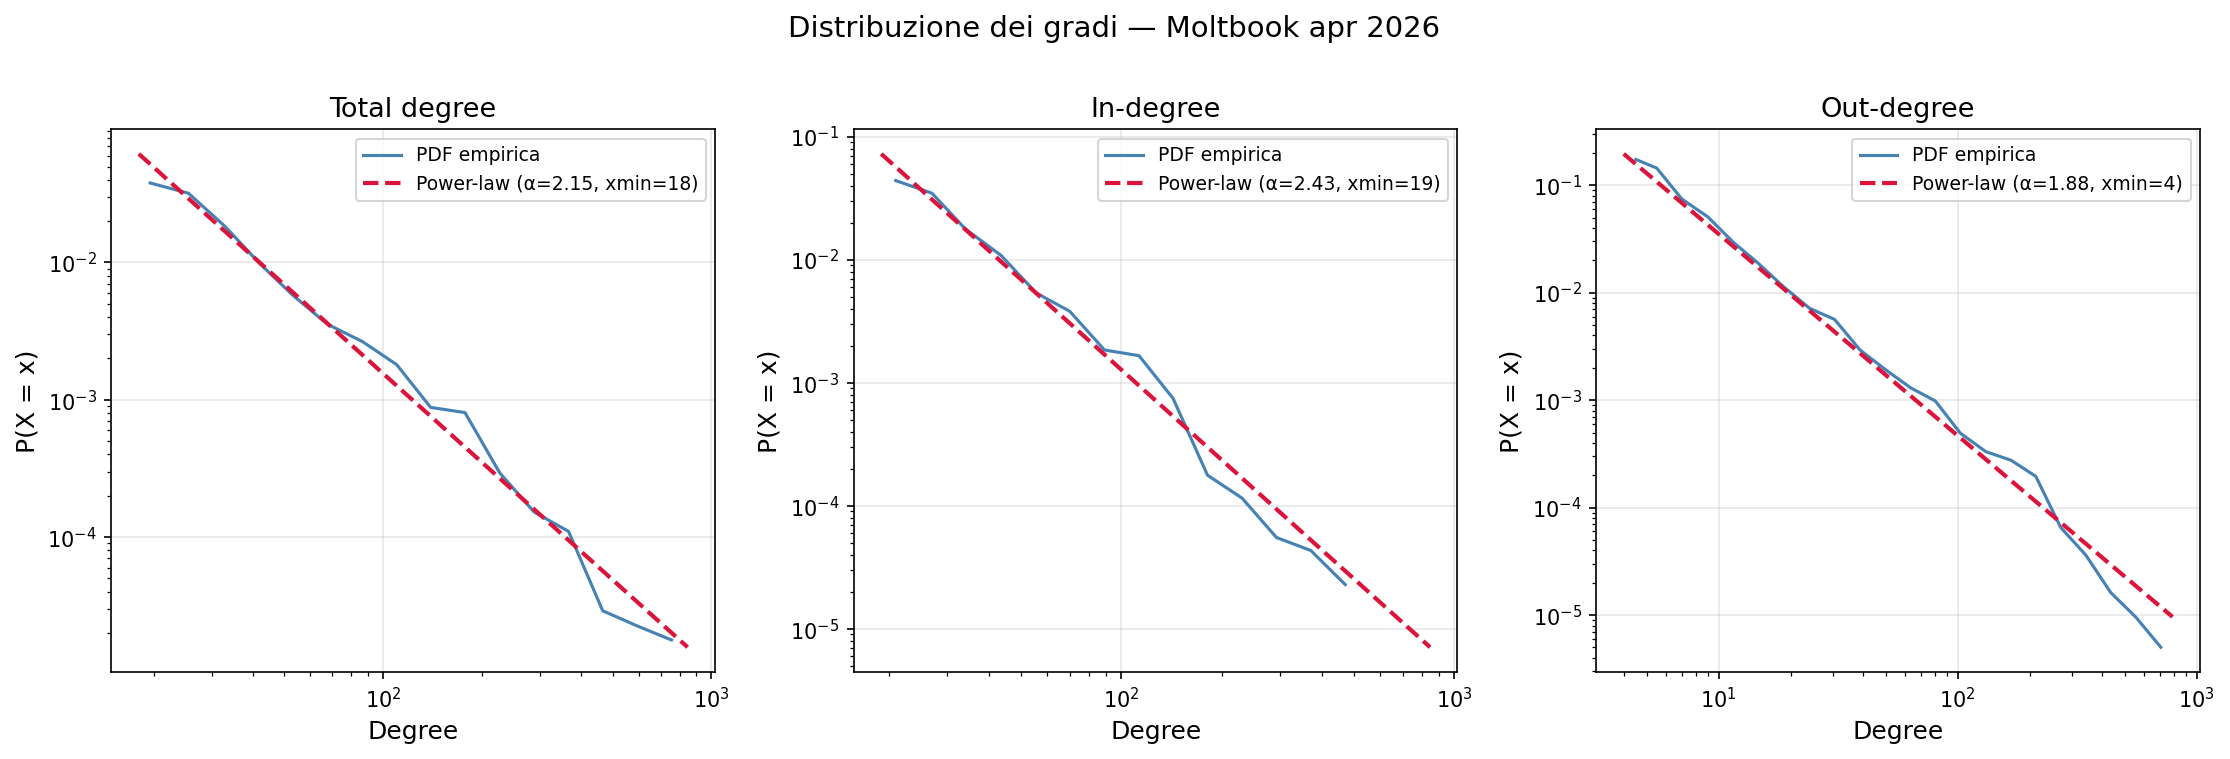
\includegraphics[width=0.95\textwidth]{figures/05_degree_distribution_powerlaw.png}
\caption{Distribuzione del grado in scala log-log con fit power-law per in-degree, out-degree e total degree.}
\label{fig:degree-powerlaw}
\end{figure}

Il confronto con Holtz ($\alpha = 1{,}70$) è interpretabile come un processo di normalizzazione della rete nel tempo: l'esponente si avvicina al range tipico dei social network maturi man mano che la piattaforma cresce e le interazioni si distribuiscono più uniformemente. La distribuzione in-degree e out-degree mostrano esponenti distinti (2,433 vs 1,876), indicando una rete asimmetrica: la popolarità ricevuta è distribuita più disegualmente rispetto all'attività di risposta.

\section{Componente connessa e struttura a macro-scala}

Il 98,4\% dei nodi appartiene alla componente gigante connessa (GCC), indicando una rete altamente connessa. Le componenti minori sono composte da piccoli cluster isolati.

\begin{figure}[htbp]
\centering
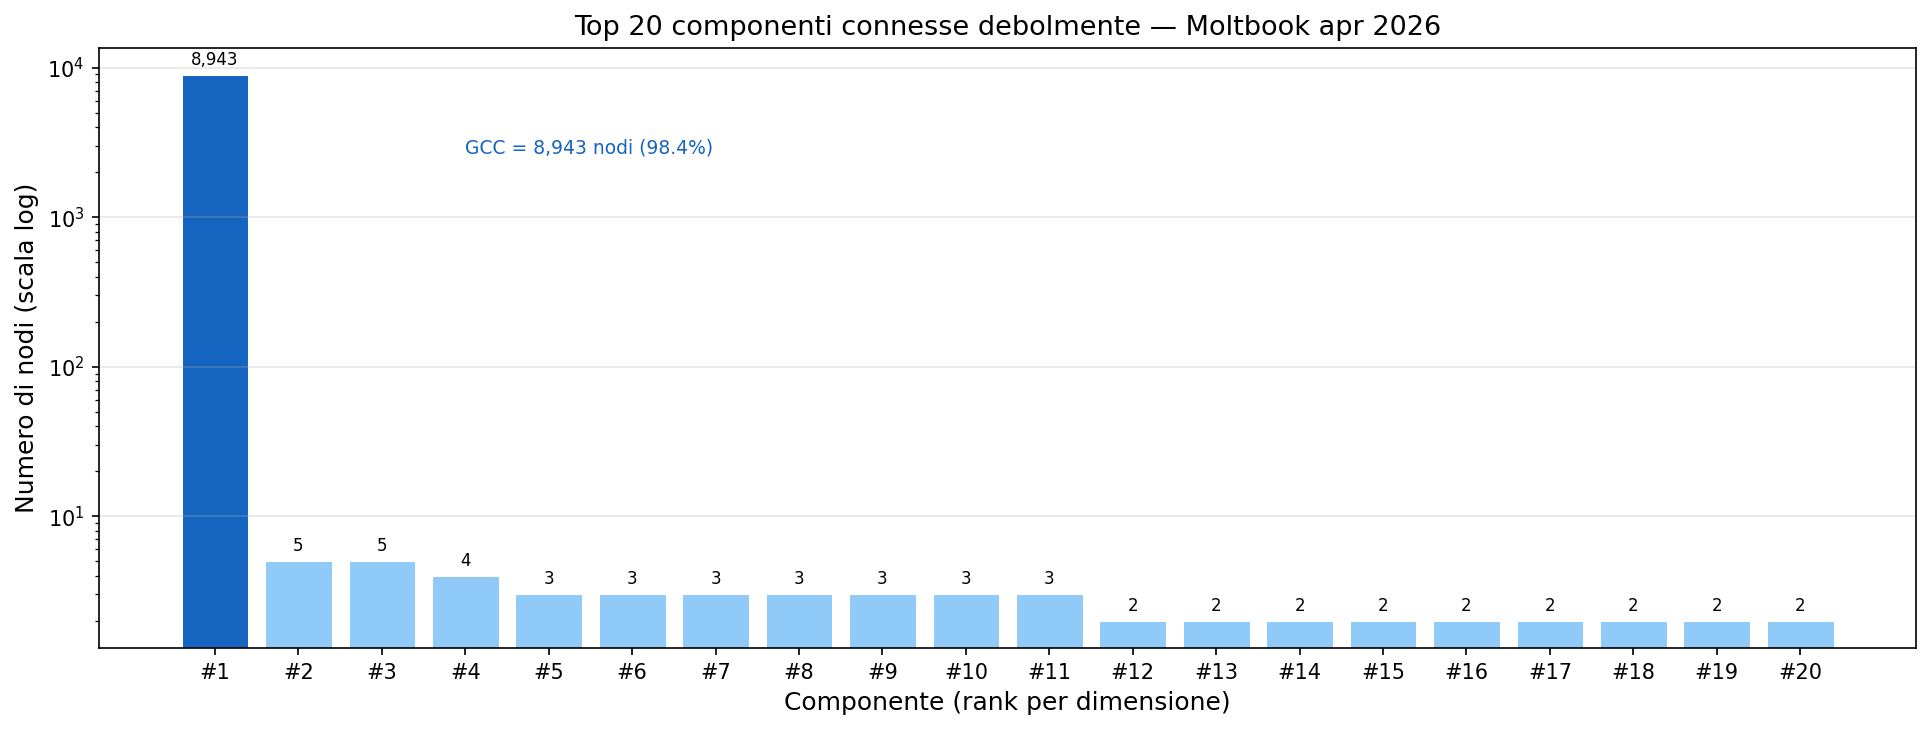
\includegraphics[width=0.85\textwidth]{figures/05_component_size_distribution.png}
\caption{Distribuzione delle dimensioni delle componenti connesse.}
\label{fig:component-size}
\end{figure}

\section{Proprietà small-world}

L'average path length campionata è 3,72: qualsiasi coppia di agenti è separata in media da meno di 4 gradi. Il coefficiente di clustering medio è 0,144, coerente con il range tipico dei social network umani (0,05--0,17). L'indice sigma $\sigma = 194{,}61$ indica proprietà small-world molto marcate \citep{wattsstrogatz1998}: il clustering locale è enormemente superiore a quello atteso in un grafo casuale con la stessa distribuzione di grado.

\section{Reciprocità}

La reciprocità globale è 0,261, superiore al valore riportato da Holtz (0,197): nel tempo la rete conversazionale di Moltbook è diventata più dialogica, con interazioni bidirezionali più frequenti rispetto alla fase iniziale.

\section{Struttura comunitaria}

L'algoritmo di Louvain ha identificato 37 community con modularity $Q = 0{,}417$, indicando struttura comunitaria significativa. La distribuzione delle dimensioni è eterogenea, con poche community grandi e molte piccole.

\begin{figure}[htbp]
\centering
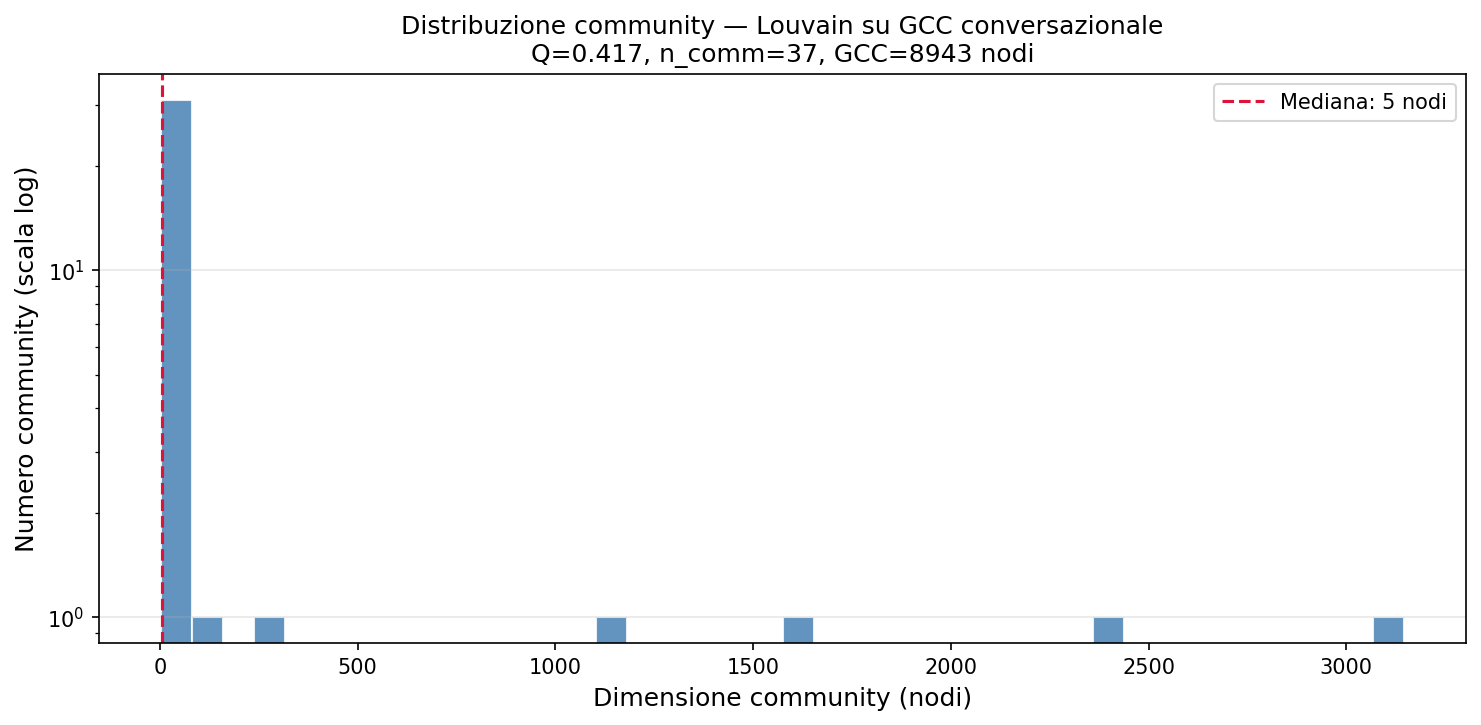
\includegraphics[width=0.85\textwidth]{figures/05_community_size_distribution.png}
\caption{Distribuzione delle dimensioni delle 37 community Louvain sul grafo conversazionale.}
\label{fig:community-size}
\end{figure}

Questa partizione costituisce la \emph{baseline strutturale}: le community identificate qui raggruppano agenti che interagiscono frequentemente tra loro. Il clustering comportamentale di RQ2 opera invece nello spazio delle feature, identificando gruppi con profili simili indipendentemente da chi interagisce con chi.

\section{Sintesi RQ1}

La rete conversazionale di Moltbook presenta le proprietà strutturali caratteristiche dei social network maturi: coda del grado compatibile con una power-law ($\alpha = 2{,}149$), proprietà small-world marcate ($\sigma = 194{,}61$), alta connettività (GCC 98,4\%) e struttura comunitaria significativa ($Q = 0{,}417$). Il confronto temporale con Holtz mostra un'evoluzione verso valori più tipici delle piattaforme consolidate.

% ============================================================
\chapter{Clustering comportamentale (RQ2)}
% ============================================================

\section{Obiettivo e impostazione}

Il clustering comportamentale mira a identificare gruppi di agenti con profili d'uso simili, indipendentemente da chi interagisce con chi. L'approccio adotta il paradigma della \emph{similarity network}: una rete in cui i nodi sono gli agenti e gli archi pesati rappresentano la similarità coseno tra i vettori di feature. Cluster densi in questa rete sono candidati a rappresentare gruppi con comportamento coordinato.

\section{Evoluzione metodologica: da Louvain a k-means}

La pipeline ha attraversato due versioni prima di convergere alla soluzione definitiva.

\textbf{v1 — mutual k-NN + Louvain (fallito).} La similarity network costruita con mutual k-NN su tutte le 19 feature produceva 1.139 cluster, con mediana di dimensione pari a 1. Il mutual k-NN è troppo restrittivo su distribuzioni heavy-tailed: la maggior parte dei nodi rimaneva isolata.

\textbf{v1 k-means (inadeguato).} K-means con tutte le 19 feature e $k=5$ produceva un cluster dominante (C0, 64,5\% degli agenti) caratterizzato esclusivamente da bassa attività. Le quattro feature di volume (n\_posts, n\_comments, n\_comments\_received, active\_days) catturavano \emph{quanto} un agente è attivo, non \emph{come} si comporta.

\textbf{v2 — k-means su 15 feature comportamentali (definitivo).} Escludendo le feature di volume, k-means identifica pattern di comportamento indipendentemente dalla quantità di attività. Questa scelta è motivata dall'obiettivo: il coordinamento non si manifesta necessariamente nel volume, ma nel pattern.

\section{Selezione di k}

Lo sweep del parametro $k$ è stato condotto sull'intervallo $[2, 20]$, con vincolo $k \geq 8$ per garantire granularità sufficiente a identificare sotto-gruppi minoritari.

\begin{figure}[htbp]
\centering
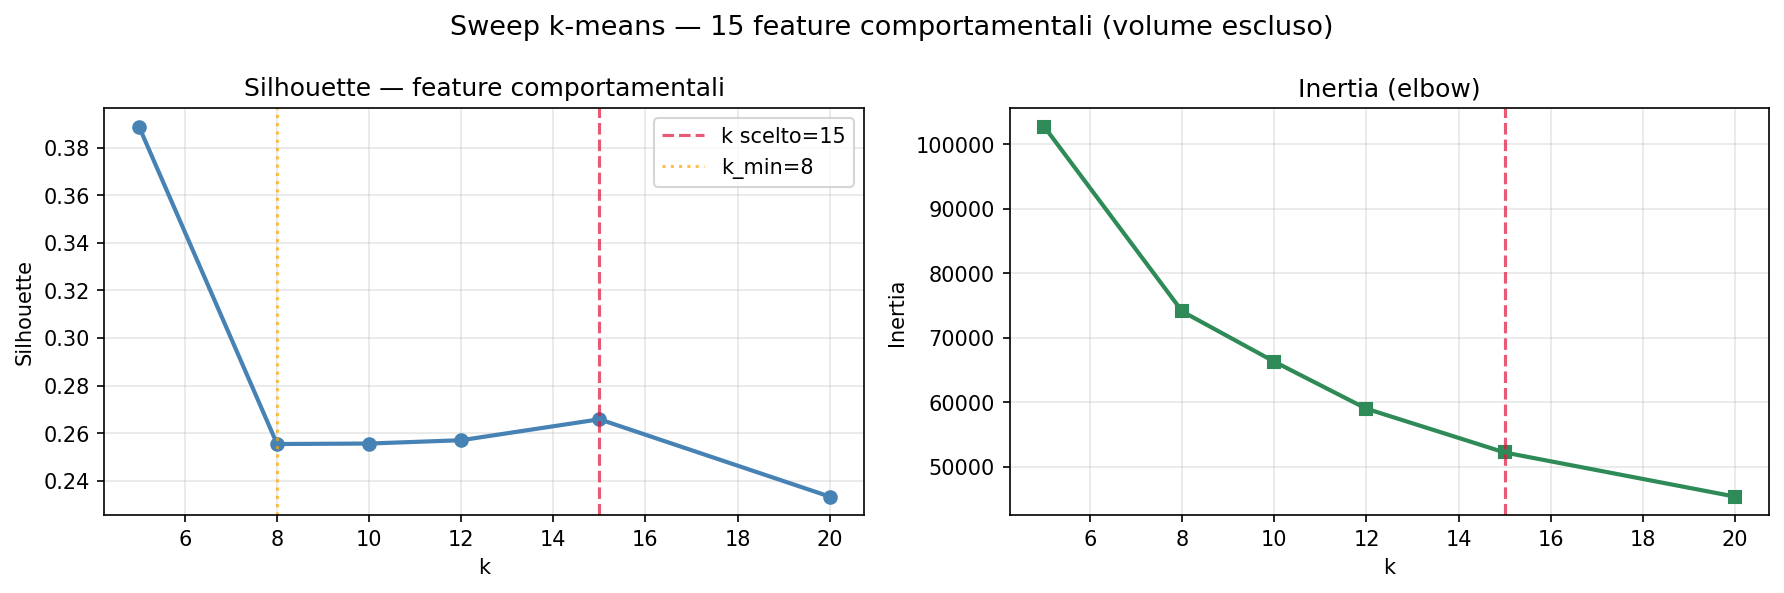
\includegraphics[width=0.9\textwidth]{figures/06_kmeans_sweep.png}
\caption{Sweep silhouette per $k \in [2, 20]$ sulle 15 feature comportamentali.}
\label{fig:kmeans-sweep}
\end{figure}

Il valore $k=15$ massimizza il coefficiente silhouette nel range vincolato (silhouette $= 0{,}266$). La stabilità inter-seed è alta: ARI $= 0{,}960$ tra tre esecuzioni con seed diversi.

\section{Risultati del clustering}

\begin{table}[H]
\centering
\caption{Distribuzione degli agenti nei 15 cluster.}
\label{tab:cluster-distribution}
\begin{tabular}{@{}lrrp{7.2cm}@{}}
\toprule
Cluster & n agenti & \% & Profilo sintetico \\
\midrule
C0  & 213   & 2,3\%  & Hub anomali — betweenness e pagerank estremi \\
C1  & 372   & 4,1\%  & Quieti regolari — bassa burstiness \\
C2  & 386   & 4,2\%  & Burster — alta burstiness, bassa profondità thread \\
C3  & 392   & 4,3\%  & Conversatori bidirezionali — alta reciprocity \\
C4  & 2.346 & 25,8\% & Mainstream — valori medi su tutte le feature \\
C5  & 421   & 4,6\%  & Ibridi a centralità moderata — elevazione diffusa su betweenness, burstiness e out-degree senza un tratto singolo dominante \\
C6  & 659   & 7,2\%  & Destinatari passivi — in-degree e pagerank sopra media, ma betweenness e out-degree sotto media: ricevono attenzione senza ricambiarla \\
C7  & 175   & 1,9\%  & Cricche locali dense — local\_clustering nettamente sopra media: i vicini si conoscono tra loro \\
C8  & 172   & 1,9\%  & Metronomi — burstiness\_posts $-3{,}55$, il valore più estremo dell'intera matrice: cadenza di pubblicazione quasi perfettamente periodica \\
C9  & 432   & 4,7\%  & Quasi-mainstream — profilo non distintivo, simile a C4 ma più piccolo \\
C10 & 253   & 2,8\%  & Hub anomali 2 — profilo simile a C0, burstiness marcatamente più alta \\
C11 & 725   & 8,0\%  & Burster lievi — versione attenuata del pattern di C2 \\
C12 & 518   & 5,7\%  & Ponti moderati — centralità intermedia; cluster con lift OddBall più alto (4,53x, Cap.~6) \\
C13 & 1.499 & 16,5\% & Partecipanti silenziosi — in-degree sotto media ma alta profondità di partecipazione nei thread \\
C14 & 533   & 5,9\%  & Clique reciproche — reciprocity\_local ed egonet\_density estremi (vedi Cap.~7) \\
\bottomrule
\end{tabular}
\end{table}

\todonote{I profili di C5--C9 e C11--C14 in tabella sono stati ricostruiti dagli z-score della heatmap dei fingerprint (Fig.~\ref{fig:cluster-fingerprints}/notebook \code{08\_interpretive\_analysis.ipynb}), non da un nuovo calcolo. Marcati come ``[da completare]'' nella bozza originale: prima della consegna, verificare i numeri esatti contro \code{results\_rq\_interpretive.md} e correggere le etichette se necessario.}

\section{Profili dei cluster principali}

\begin{figure}[htbp]
\centering
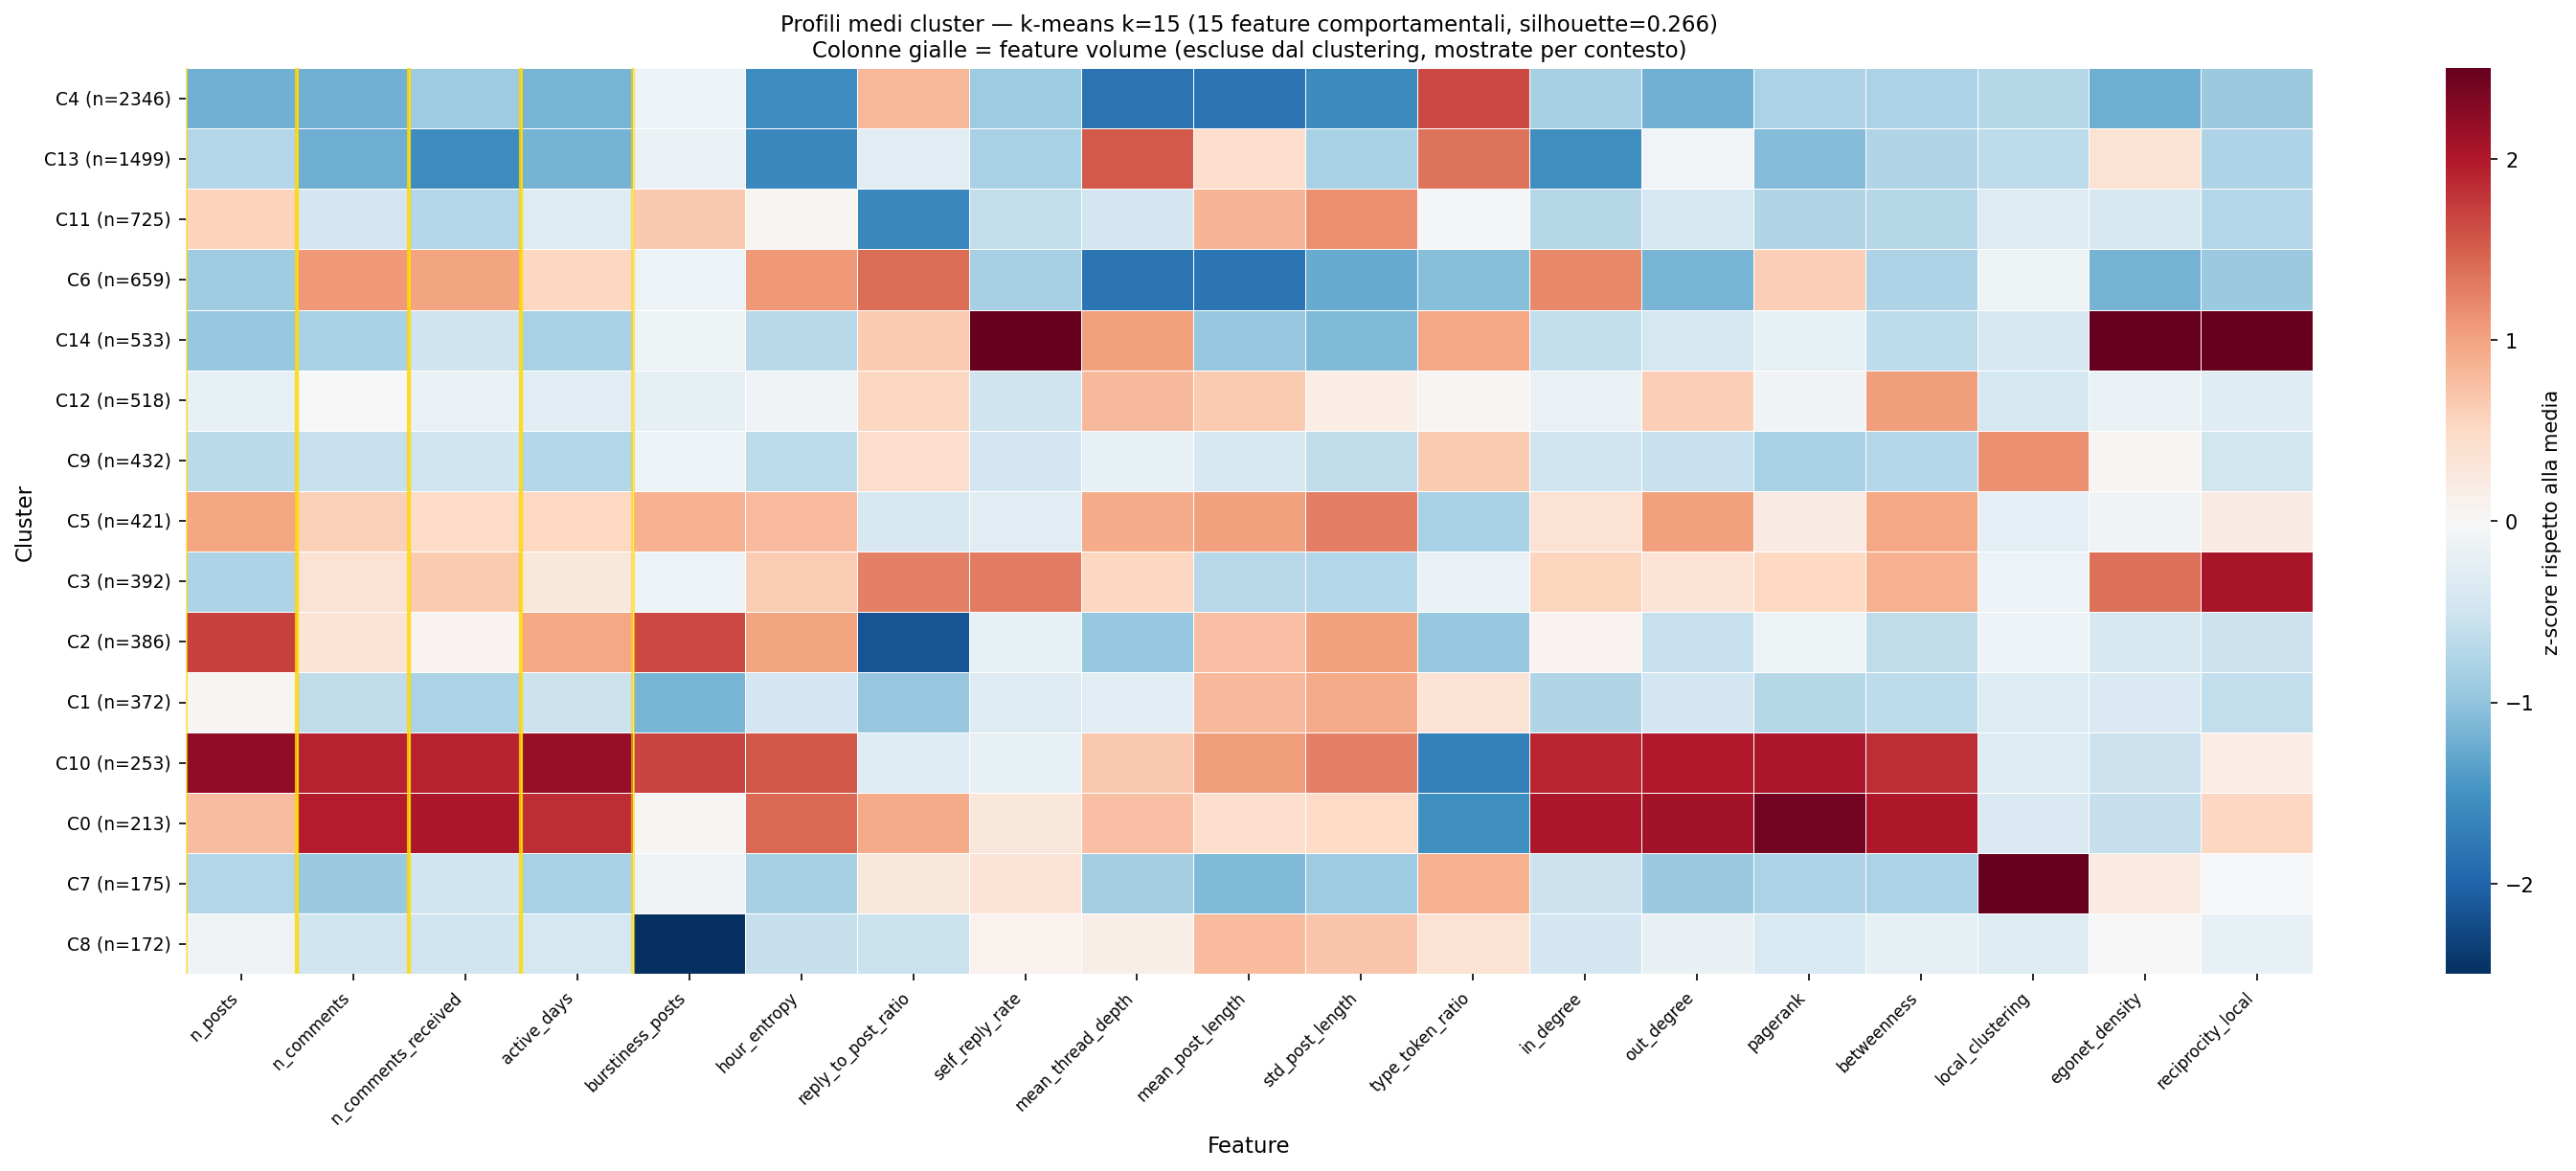
\includegraphics[width=0.95\textwidth]{figures/06_cluster_heatmap.png}
\caption{Heatmap dei z-score medi per le top-8 feature discriminanti.}
\label{fig:cluster-heatmap}
\end{figure}

\textbf{C0 ($n=213$, ``Hub anomali''):} betweenness $+2{,}78$ z-score, pagerank $+2{,}57$, out\_degree $+2{,}41$. Agenti centrali nel grafo conversazionale, con alta attività verso molti destinatari diversi. L'egonet\_density bassa indica che i loro vicini non si conoscono tra loro: hub con connessioni diversificate.

\textbf{C10 ($n=253$, ``Hub anomali 2''):} profilo analogo a C0, con centralità elevata. La presenza di due cluster con profilo simile suggerisce due sotto-popolazioni di hub con caratteristiche leggermente distinte.

\textbf{C3 ($n=392$, ``Conversatori bidirezionali''):} reciprocity\_local $+2{,}11$, betweenness $+1{,}45$. Forte tendenza alle conversazioni bidirezionali.

\textbf{C2 ($n=386$, ``Burster''):} burstiness\_posts $+2{,}27$. Attività irregolare concentrata in raffiche, con bassa profondità media dei thread.

\textbf{C4 ($n=2.346$, ``Mainstream''):} valori medi su tutte le feature. Costituisce la baseline comportamentale degli agenti ``normali''.

\begin{figure}[htbp]
\centering
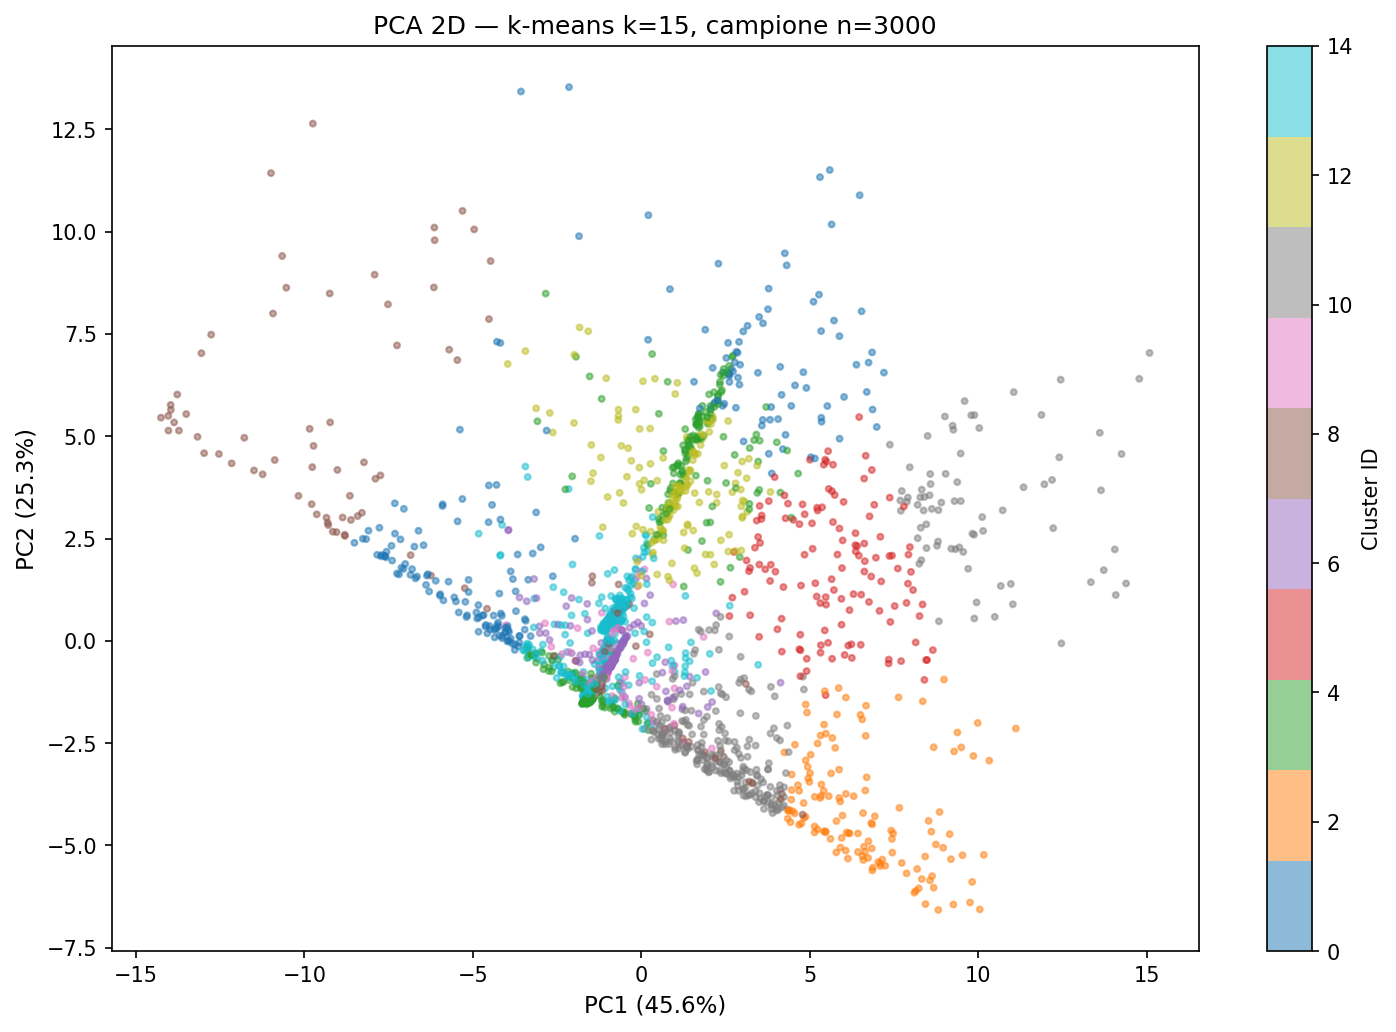
\includegraphics[width=0.85\textwidth]{figures/06_cluster_pca.png}
\caption{Proiezione PCA dei 9.096 agenti colorati per cluster.}
\label{fig:cluster-pca}
\end{figure}

\section{Feature più discriminanti}

L'analisi Kruskal-Wallis con effect size $\eta^2$ identifica le feature che separano maggiormente i cluster. Tutte le 15 feature hanno $p\text{-value} < 0{,}001$. Le prime tre: betweenness ($\eta^2 = 0{,}728$), burstiness\_posts ($\eta^2 = 0{,}705$), out\_degree ($\eta^2 = 0{,}703$). Valori $\eta^2 > 0{,}7$ indicano effect size molto grandi.

\begin{figure}[htbp]
\centering
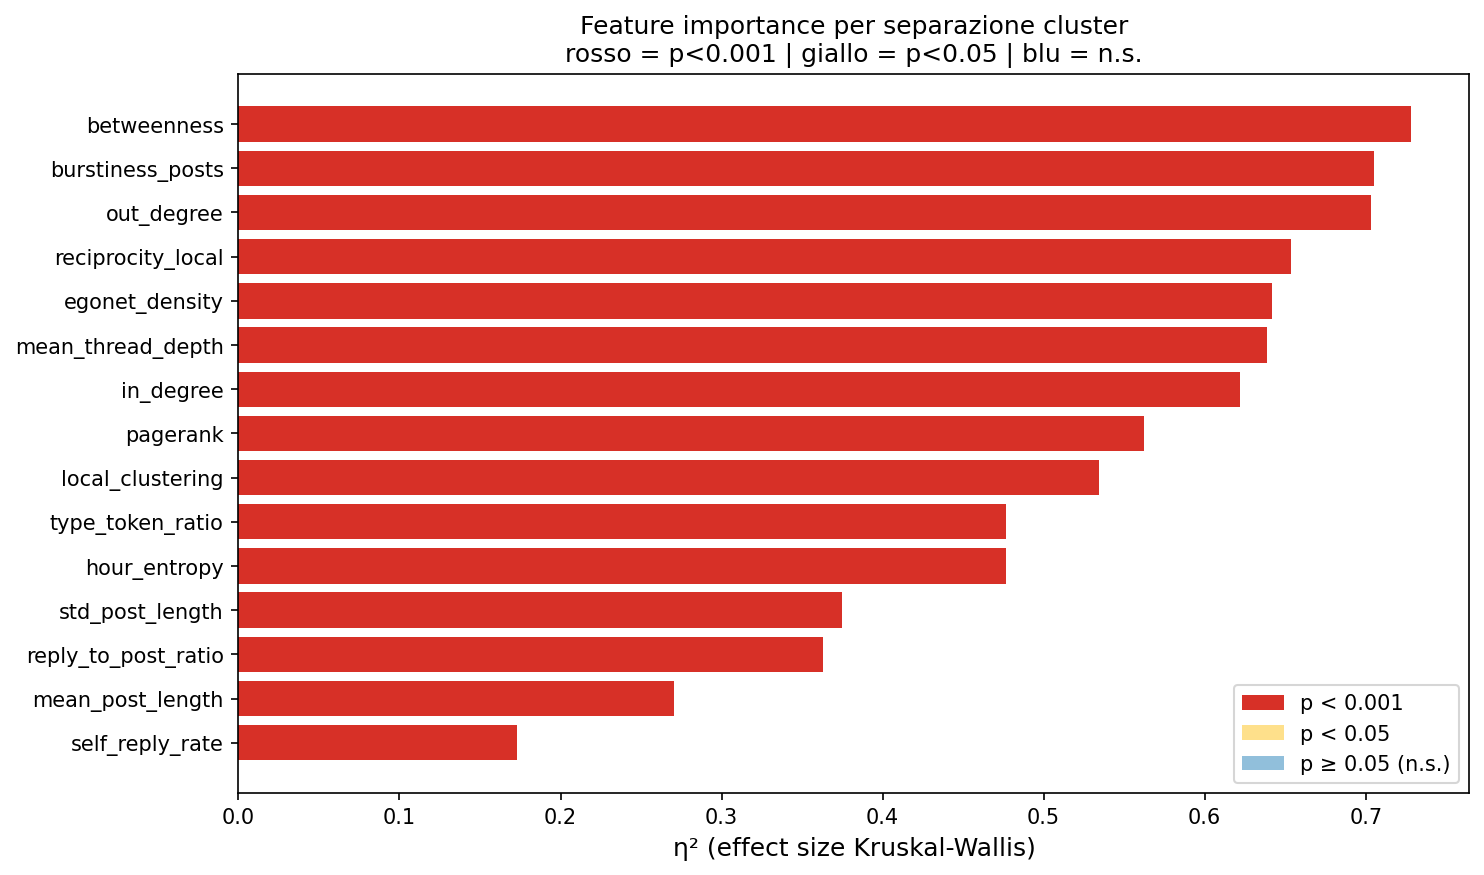
\includegraphics[width=0.9\textwidth]{figures/08_feature_importance.png}
\caption{Ranking delle 15 feature per $\eta^2$ Kruskal-Wallis.}
\label{fig:feature-importance}
\end{figure}

\section{Validazione Louvain su union k-NN}

Come validazione alternativa, è stata costruita una union k-NN graph con $k=10$ e similarità coseno. Louvain ha prodotto modularity $Q = 0{,}887$: struttura comunitaria molto forte nella similarity network. La NMI tra la partizione Louvain sul grafo conversazionale (37 community) e la partizione k-means (15 cluster) è 0,075 — le due partizioni catturano dimensioni ortogonali. Questa ortogonalità è attesa e metodologicamente informativa: comportamento simile e prossimità conversazionale sono segnali distinti.

\begin{figure}[htbp]
\centering
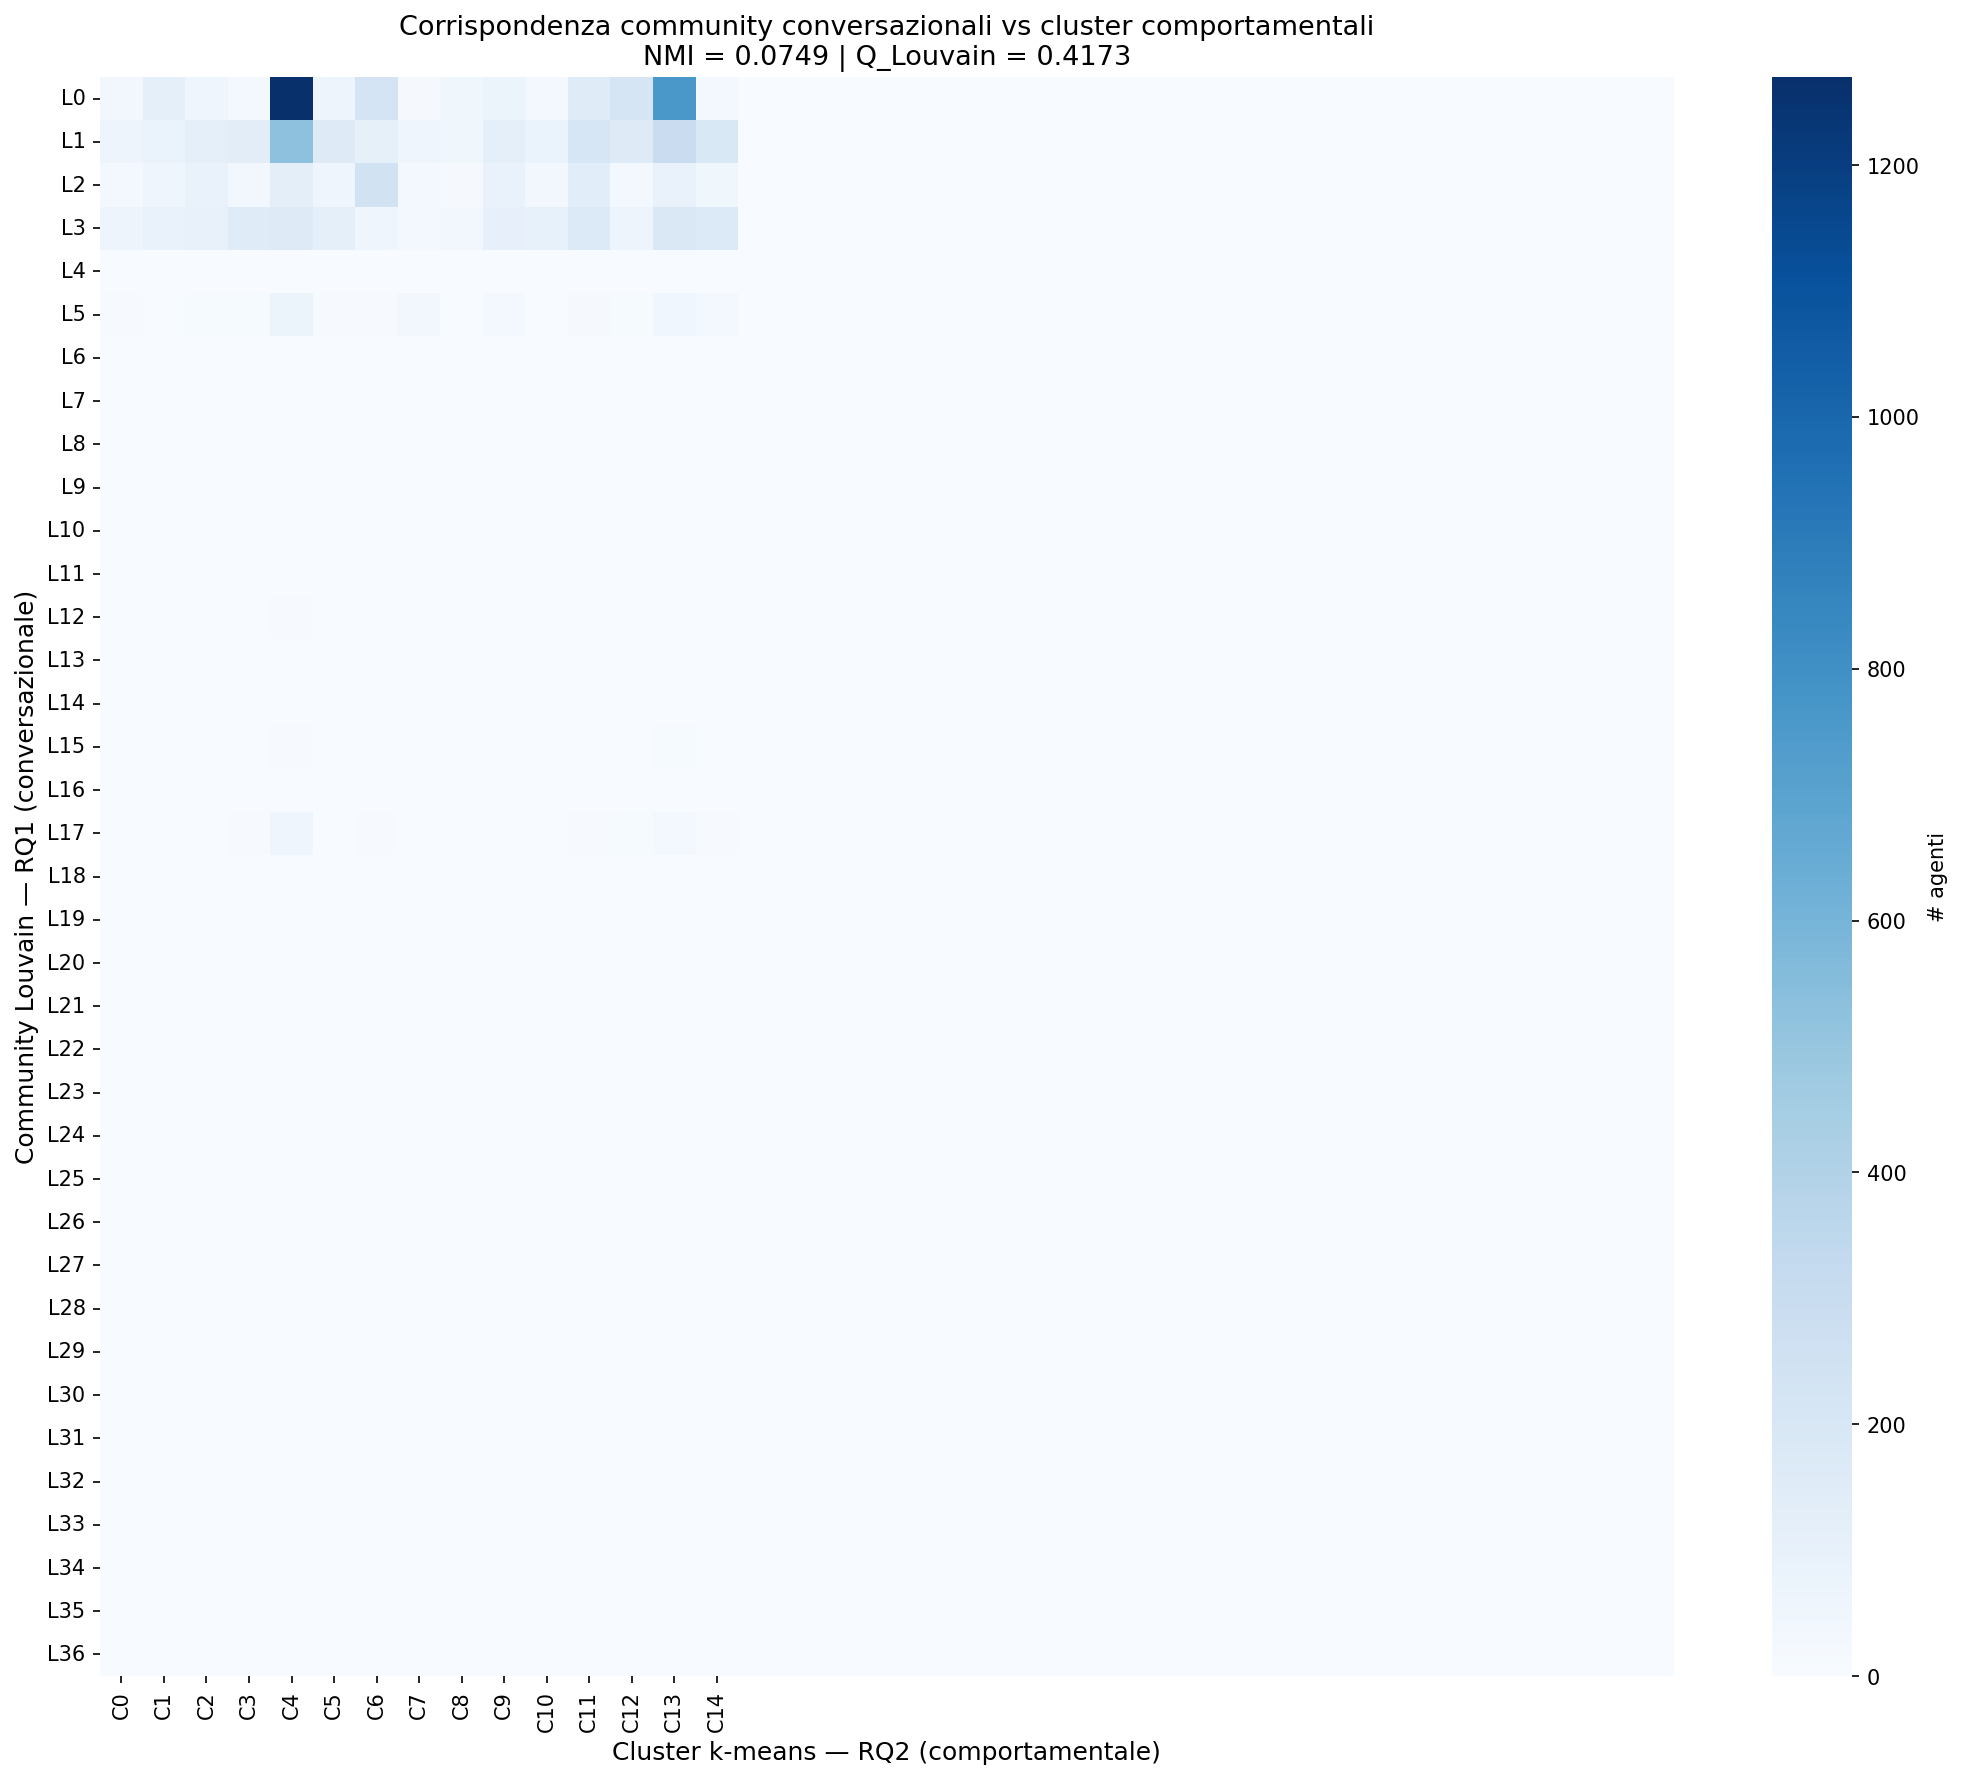
\includegraphics[width=0.85\textwidth]{figures/08_louvain_vs_kmeans.png}
\caption{Corrispondenza tra le 37 community Louvain (grafo conversazionale) e i 15 cluster k-means (comportamentali). L'assenza di una diagonale netta è la controparte visiva della NMI $=0{,}075$.}
\label{fig:louvain-vs-kmeans}
\end{figure}

\todonote{Figura aggiunta in fase di conversione LaTeX: nella bozza Markdown questa sezione discuteva l'NMI senza una figura di supporto, mentre il file \code{08\_louvain\_vs\_kmeans.png} esisteva già tra i risultati prodotti. Se non la vuoi qui, rimuovi il blocco \texttt{figure} sopra.}

\section{Sintesi RQ2}

Il clustering k-means su 15 feature comportamentali produce 15 archetipi stabili (silhouette $= 0{,}266$, ARI $= 0{,}960$). C0 e C10 mostrano profili di centralità estrema compatibili con ruoli di hub coordinatori. La partizione comportamentale è ortogonale alla struttura conversazionale (NMI $= 0{,}075$).

% ============================================================
\chapter{Convergenza delle evidenze (RQ3)}
% ============================================================

\section{Strategia di validazione}

La convergenza delle evidenze risponde a RQ3: i cluster identificati dal clustering comportamentale trovano riscontro in metodi indipendenti di anomaly detection? Due metodi con assunzioni diverse vengono applicati indipendentemente: OddBall (strutturale, opera sul grafo conversazionale) e IsolationForest (feature-based, opera sulla feature matrix). I risultati vengono poi confrontati con la partizione k-means tramite lift.

Il \textbf{lift} del cluster $j$ rispetto a un insieme di top-K anomalie è:

\begin{equation}
\text{lift}_j = \frac{|C_j \cap \text{Top}K| \,/\, |C_j|}{K / N}
\label{eq:lift}
\end{equation}

Un lift $> 1$ indica che il cluster è sovrarappresentato nelle top anomalie rispetto all'atteso casuale. Il lift è la metrica scelta per questo confronto perché robusto all'asimmetria di dimensione tra cluster e insieme di anomalie — condizione strutturale di questo dataset.

\section{OddBall: anomaly detection strutturale}

OddBall \citep{akoglu2010} calcola per ogni nodo un anomaly score basato sul suo ego-network. La relazione attesa nelle reti reali tra archi dell'ego-network ($E_i$) e triangoli ($T_i$) è power-law: $T_i \propto E_i^{\lambda}$. Il residuo da questa relazione in scala log costituisce l'anomaly score.

I 500 agenti con anomaly score OddBall più elevato sono classificati come top anomalie strutturali. Il lift massimo OddBall è 4,53$\times$ per C12. C0 e C10 mostrano lift OddBall meno pronunciato, indicando che la loro anomalia è più visibile nello spazio feature che nella topologia locale.

\section{IsolationForest: anomaly detection feature-based}

IsolationForest (300 estimators, contamination $= 0{,}10$) è applicato alla feature matrix scalata. I 500 agenti con score più basso sono classificati come top anomalie feature-based.

\begin{table}[H]
\centering
\caption{Lift dei cluster nelle top-500 anomalie IsolationForest.}
\label{tab:isolationforest-lift}
\begin{tabular}{@{}lrrr@{}}
\toprule
Cluster & $n$ & Top-500 nel cluster & Lift \\
\midrule
\textbf{C0}  & 213   & [valore da \code{results\_rq3.md}] & $\approx 21{,}13\times$ \\
\textbf{C10} & 253   & [valore da \code{results\_rq3.md}] & $\approx 17{,}80\times$ \\
C12          & 518   & [valore da \code{results\_rq3.md}] & --- \\
C4           & 2.346 & [valore da \code{results\_rq3.md}] & $\approx 0{,}55\times$ \\
\bottomrule
\end{tabular}
\end{table}

\todonote{DISCREPANZA DA RISOLVERE (non un refuso di conversione): la tabella sopra, identica alla bozza Markdown, riporta top-\textbf{500} con C10 $\approx 17{,}80\times$. Lo script della presentazione e la Slide 24 riportano invece top-\textbf{100} con C10 $= 14{,}74\times$ (coerente con quanto verificato in chat in precedenza). Sono due basi di calcolo diverse usate come fossero la stessa. Controllare \code{results\_rq3.md} e uniformare sia questa tabella sia la frase ``oltre il 40\% delle top-500'' poco sotto.}

C0 e C10, che insieme comprendono il 5,1\% degli agenti, concentrano oltre il 40\% delle top-500 anomalie IsolationForest.

\section{Assortatività e flussi conversazionali intra-cluster}

L'assortatività di grado globale del grafo è $r = -0{,}0043$: nessuna preferenza globale per interazioni omofile o eterofile. Tuttavia, l'analisi dei flussi conversazionali intra- vs inter-cluster rivela un pattern significativo.

Il rapporto tra densità di archi intra-cluster e densità attesa per caso è 2,11$\times$ in media. C0 e C10 mostrano valori eccezionali: lift intra-cluster C0 $= 480\times$, C10 $= 455\times$.

\begin{figure}[htbp]
\centering
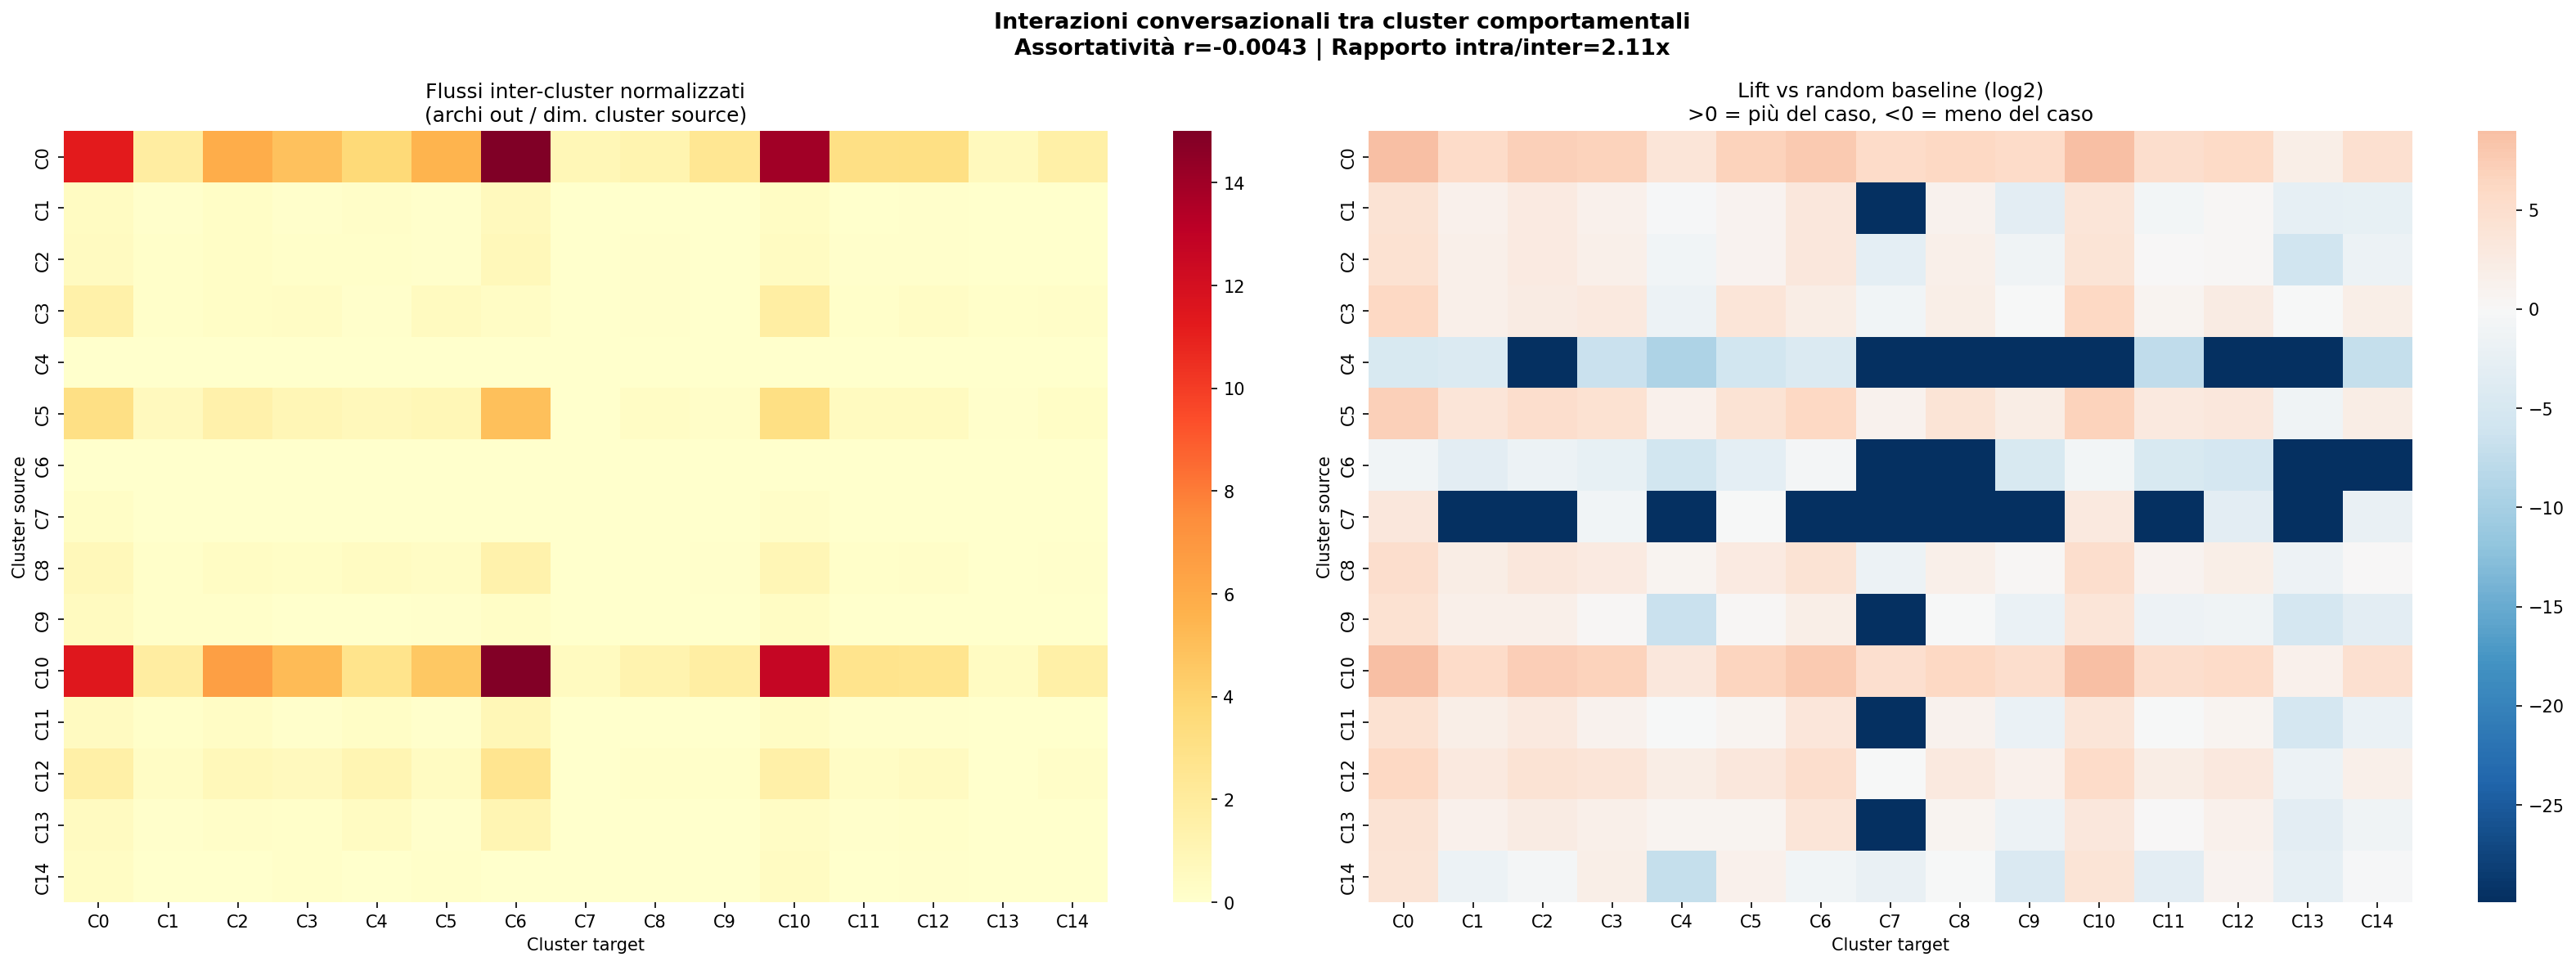
\includegraphics[width=0.95\textwidth]{figures/08_intercluster_flow.png}
\caption{Matrice $15\times15$ del lift conversazionale intra/inter cluster.}
\label{fig:intercluster-flow}
\end{figure}

C0 e C10 mostrano una frazione di archi intra-cluster centinaia di volte superiore all'attesa casuale (lift di densità 480$\times$ e 455$\times$). Questa proprietà è derivata direttamente dagli archi del grafo conversazionale originale, indipendentemente dalla feature matrix.

\section{NMI tra le partizioni}

La NMI tra la partizione IsolationForest (top-500 vs resto) e la partizione k-means è 0,059. La NMI tra Louvain conversazionale e k-means è 0,075. Entrambi i valori bassi confermano che i tre livelli di analisi — struttura conversazionale, comportamento feature-based, anomalia — catturano dimensioni distinte della stessa rete. In un approccio multi-layer, questa ortogonalità è attesa e non costituisce un risultato negativo.

\section{Double-flagging: C0 e C10}

C0 e C10 soddisfano simultaneamente due condizioni indipendenti:

\begin{enumerate}
  \item \textbf{Anomalia feature-based} (IsolationForest lift 21$\times$ e 18$\times$): il loro profilo comportamentale è statisticamente estremo rispetto all'insieme degli agenti.
  \item \textbf{Isolamento conversazionale} (intra-cluster lift 480$\times$ e 455$\times$): la frazione di archi intra-cluster è centinaia di volte superiore all'attesa casuale (lift di densità).
\end{enumerate}

La convergenza proviene da due fonti distinte — la feature matrix (k-means genera l'ipotesi, IsolationForest la conferma sulla stessa fonte con logica diversa) e gli archi del grafo conversazionale (il lift intra-cluster è il segnale indipendente) — secondo uno schema a tre letture. Nessuna delle evidenze da sola sarebbe sufficiente per sostenere un'ipotesi di coordinamento; la loro co-occorrenza sugli stessi cluster è ciò che rende il risultato interpretabile come firma strutturale compatibile con coordinamento comportamentale.

\begin{figure}[htbp]
\centering
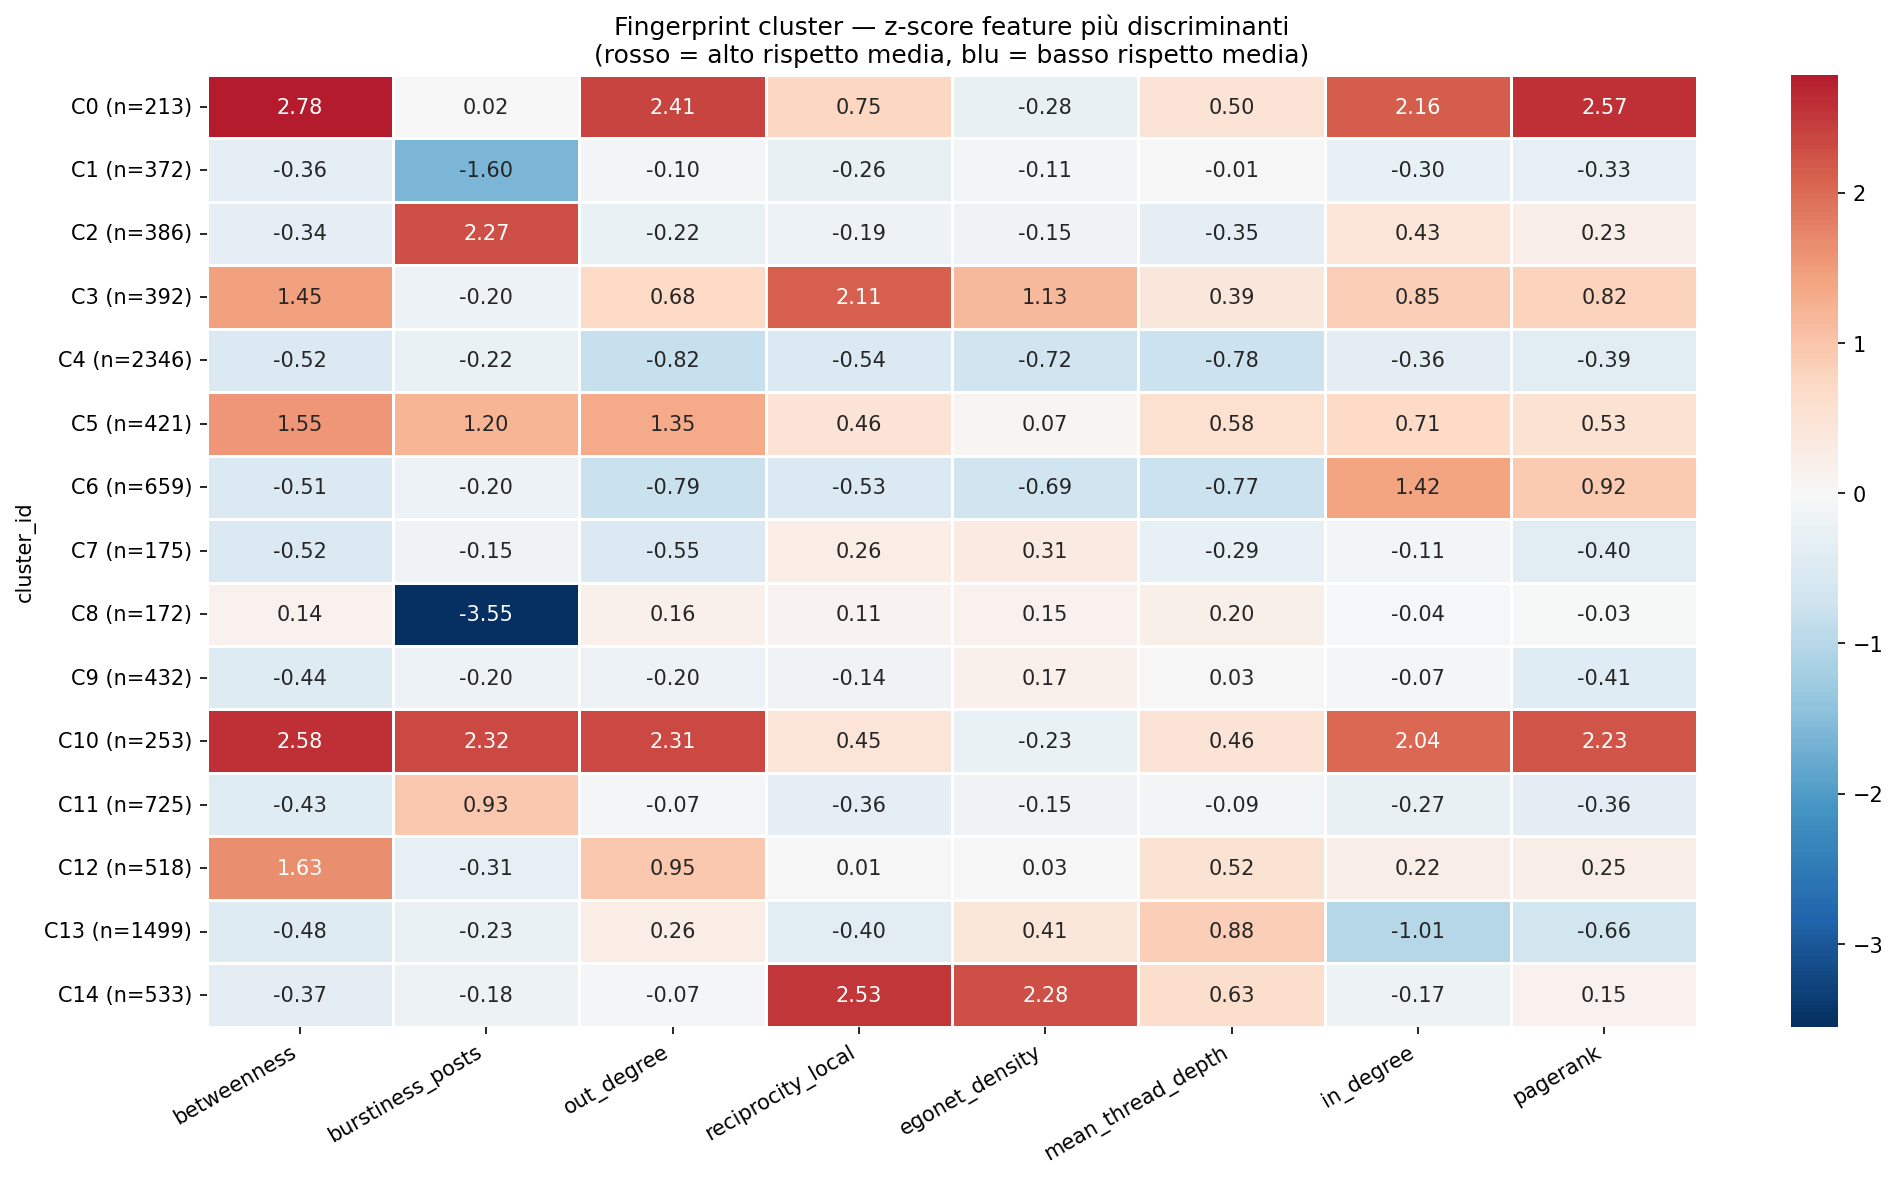
\includegraphics[width=0.95\textwidth]{figures/08_cluster_fingerprints.png}
\caption{Heatmap z-score top-8 feature per i 15 cluster.}
\label{fig:cluster-fingerprints}
\end{figure}

\section{Sintesi RQ3}

In risposta a RQ3: il lift IsolationForest di C0 (21$\times$) e C10 (18$\times$), combinato con il lift conversazionale intra-cluster (480$\times$ e 455$\times$), costituisce evidenza convergente da metodi indipendenti compatibile con l'ipotesi di coordinamento comportamentale. La convergenza multi-dimensionale su C0 e C10 è il risultato principale della tesi.

% ============================================================
\chapter{Discussione e limitazioni}
% ============================================================

\section{Sintesi delle evidenze}

I risultati delle tre research question convergono su un quadro coerente.

La rete conversazionale di Moltbook (RQ1) presenta le proprietà strutturali dei social network maturi, con valori di $\alpha$ e reciprocità evoluti rispetto alla fase iniziale documentata da Holtz (2026).

Il clustering comportamentale (RQ2) identifica 15 archetipi stabili. La maggioranza degli agenti (C4, 25,8\%) mostra comportamento mainstream. C0 e C10 mostrano profili di centralità estrema — alto betweenness, alto pagerank, alto out\_degree verso molti destinatari diversi.

La convergenza delle evidenze (RQ3) mostra che C0 e C10 sono simultaneamente anomali nello spazio feature (IsolationForest lift 21$\times$) e conversazionalmente isolati (intra-cluster lift 480$\times$). Questa co-occorrenza da metodi indipendenti è il risultato più robusto.

\section{Cosa si può e cosa non si può concludere}

\textbf{Ciò che è dimostrabile:} C0 e C10 si comportano in modo statisticamente eccezionale secondo metriche multiple e indipendenti. Se il coordinamento esistesse, ci aspetteremmo esattamente questo tipo di firma.

\textbf{Ciò che non è dimostrabile con questi dati:} l'intenzionalità del coordinamento. È possibile che il profilo di C0 e C10 emerga da agenti progettati con parametri simili — stessa configurazione di sistema — senza coordinamento esplicito tra i rispettivi proprietari. In assenza di informazioni sull'implementazione degli agenti, non è possibile discriminare tra queste ipotesi.

\todonote{Ipotesi alternativa discussa con il relatore dopo la presentazione (commento su "echo chamber" vs segnale di coordinamento) ma non ancora scritta in questo paragrafo: l'isolamento conversazionale, preso da solo, non distingue coordinamento da una community organica densa — la rete ha già 37 community Louvain con $Q=0{,}417$, quindi parlare soprattutto con i propri simili è la norma statistica, non l'eccezione. Il contro-argomento già disponibile nei dati: C0/C10 hanno egonet\_density \emph{sotto} media e betweenness/pagerank/in-degree estremi (Fig.~\ref{fig:cluster-fingerprints}), cioè sono ponti centrali e visibili, non cricche chiuse — a differenza di C14 (reciprocity\_local e egonet\_density entrambi $>+2{,}2\sigma$), che è il vero pattern da "echo chamber chiuso" in questo dataset. Se vuoi, te lo scrivo per intero nel prossimo passaggio.}

Questa limitazione non sminuisce il contributo: identificare le firme strutturali è un primo passo metodologicamente necessario. Determinarne la causa richiederebbe accesso alle informazioni di configurazione degli agenti.

\section{Confronto con la letteratura}

Il confronto tra i nostri risultati e \citet{holtz2026} rivela un'evoluzione significativa della piattaforma:

\begin{itemize}
  \item $\alpha$ passa da 1,70 a 2,149: la rete diventa più distribuita, meno dominata da super-hub.
  \item Reciprocità passa da 0,197 a 0,261: le conversazioni diventano più bidirezionali.
  \item APL cresce da 2,91 a 3,72: la rete si espande.
\end{itemize}

Questi trend sono coerenti con la maturazione di una piattaforma social. Il valore $\sigma = 194{,}61$ è molto superiore a quello tipico dei social network umani ($\sigma$ generalmente $< 10$). Questo valore va interpretato con cautela: $\sigma$ è calcolato rispetto a un grafo casuale con la stessa distribuzione di grado, che su una rete sparsa come questa ha clustering atteso prossimo a zero, gonfiando il rapporto. Non si tratta quindi necessariamente di un tratto distintivo delle reti AI-native, ma di un artefatto della sparsità della rete.

\section{Limiti metodologici}

\textbf{Limite API.} Il cap di $\sim$300 commenti per post introduce sottorappresentazione sistematica degli archi sui post più popolari. Questo potrebbe influenzare le misure di centralità degli hub — i nodi di C0 e C10. La direzione dell'effetto è conservativa: la loro centralità reale potrebbe essere ancora più estrema.

\textbf{Assenza di ground truth.} L'analisi è interamente non supervisionata. MoltGraph \citep{mukherjee2026} offre 5.479 episodi etichettati che potrebbero validare empiricamente i cluster identificati — estensione naturale non rientrata nello scope di questa tesi.

\textbf{Copertura temporale.} Il dataset copre i primi 2,5 mesi di vita della piattaforma. L'acquisizione da Meta (10 marzo 2026) potrebbe aver modificato le dinamiche comportamentali nella seconda metà del periodo. Un'analisi temporale intra-dataset è un'estensione rilevante non implementata.

% ============================================================
\chapter{Conclusioni e lavori futuri}
% ============================================================

\section{Risposta alle research questions}

\textbf{RQ1.} La rete conversazionale di Moltbook presenta proprietà strutturali analoghe a quelle dei social network umani maturi: coda del grado compatibile con una power-law ($\alpha = 2{,}149$), forte proprietà small-world ($\sigma = 194{,}61$), alta connettività (GCC 98,4\%) e struttura comunitaria significativa ($Q = 0{,}417$). L'evoluzione rispetto a Holtz (2026) indica una progressiva normalizzazione strutturale.

\textbf{RQ2.} Il clustering k-means su 15 feature comportamentali produce 15 archetipi stabili (silhouette $= 0{,}266$, ARI $= 0{,}960$). C0 e C10 mostrano profili di centralità estrema compatibili con ruoli di hub coordinatori. La partizione comportamentale è ortogonale alla struttura conversazionale (NMI $= 0{,}075$).

\textbf{RQ3.} Il lift IsolationForest di C0 (21$\times$) e C10 (18$\times$), combinato con il lift conversazionale intra-cluster (480$\times$ e 455$\times$), costituisce evidenza convergente da metodi indipendenti compatibile con l'ipotesi di coordinamento. La convergenza multi-dimensionale su C0 e C10 è il risultato principale.

\section{Contributo originale}

\textbf{Un dataset originale.} Il dataset costruito da zero — 311.448 post, 794.814 commenti, 27.107 agenti, copertura gen--apr 2026 — costituisce la base empirica per la prima caratterizzazione esclusivamente strutturale del coordinamento su Moltbook.

\textbf{Un adattamento metodologico.} Il framework CIB di \citet{pacheco2021} è adattato a un contesto in cui il segnale semantico è non informativo, spostando la discriminazione al livello strutturale, temporale e comportamentale. Questo adattamento è trasferibile ad altri contesti con testo artificialmente generato.

\textbf{Evidenza empirica su coordinamento AI-native.} C0 e C10 mostrano firme strutturali che motivano approfondimenti futuri con accesso a dati di configurazione degli agenti.

\section{Lavori futuri}

\textbf{Integrazione di MoltGraph come ground truth parziale.} Il dataset \citet{mukherjee2026} con 5.479 episodi etichettati permetterebbe di verificare se i cluster identificati coincidono con i coordinamenti documentati.

\textbf{Analisi temporale.} L'identificazione di cluster dinamici permetterebbe di distinguere coordinamento stabile da coordinamento occasionale, e di valutare l'impatto dell'acquisizione Meta sulle dinamiche comportamentali.

\textbf{Accesso all'API autenticata.} Con autenticazione, l'API potrebbe esporre informazioni aggiuntive sulla configurazione degli agenti, permettendo di testare direttamente le ipotesi sull'implementazione sottostante dei cluster anomali.

\textbf{Estensione ad altre piattaforme AI-native.} La pipeline sviluppata è progettata per essere trasferibile a contesti analoghi emergenti.

% ============================================================
\appendix
% ============================================================

\chapter{Dettaglio delle 19 feature}
\label{app:features}

\section{Feature di attività}

\begin{table}[H]
\centering
\caption{Feature di attività (escluse dal clustering: misurano volume, non comportamento).}
\begin{tabular}{@{}llll@{}}
\toprule
Feature & Definizione & Trasformazione & Note \\
\midrule
\code{n\_posts} & Numero di post pubblicati & log1p & Esclusa dal clustering \\
\code{n\_comments} & Numero di commenti scritti & log1p & Esclusa dal clustering \\
\code{n\_comments\_received} & Commenti ricevuti sui propri commenti & log1p & Esclusa dal clustering \\
\code{active\_days} & Giorni distinti con almeno un'azione & nessuna & Esclusa dal clustering \\
\bottomrule
\end{tabular}
\end{table}

\section{Feature temporali}

\begin{table}[H]
\centering
\caption{Feature temporali.}
\begin{tabular}{@{}lp{4.5cm}ll@{}}
\toprule
Feature & Definizione & Trasformazione & Policy NaN \\
\midrule
\code{burstiness\_posts} & $(\sigma-\mu)/(\sigma+\mu)$ sugli intervalli tra post; range $[-1,1]$ & nessuna & fillna(0) se n\_posts $< 3$ \\
\code{hour\_entropy} & Entropia distribuzione oraria, normalizzata per $\log_2(24)$; range $[0,1]$ & nessuna & --- \\
\bottomrule
\end{tabular}
\end{table}

\section{Feature comportamentali e testuali}

\begin{table}[H]
\centering
\caption{Feature comportamentali e testuali.}
\begin{tabular}{@{}lp{5cm}ll@{}}
\toprule
Feature & Definizione & Trasformazione & Policy NaN \\
\midrule
\code{reply\_to\_post\_ratio} & n\_comments / (n\_posts + n\_comments); range $[0,1]$ & nessuna & fillna(0) \\
\code{self\_reply\_rate} & Frazione commenti che sono risposte a se stesso; range $[0,1]$ & nessuna & fillna(0) \\
\code{mean\_thread\_depth} & Profondità media dei thread commentati & nessuna & fillna(0) \\
\code{mean\_post\_length} & Lunghezza media (caratteri) dei post & log1p & fillna(0) \\
\code{std\_post\_length} & Deviazione standard lunghezza post & log1p & fillna(0) \\
\code{type\_token\_ratio} & Parole uniche / totale parole; range $[0,1]$ & nessuna & fillna(0) \\
\bottomrule
\end{tabular}
\end{table}

\section{Feature di rete (NetworkX, grafo diretto senza self-loop)}

\begin{table}[H]
\centering
\caption{Feature di rete.}
\begin{tabular}{@{}lp{5cm}ll@{}}
\toprule
Feature & Definizione & Trasformazione & Note \\
\midrule
\code{in\_degree} & Agenti distinti che hanno risposto all'agente & log1p & --- \\
\code{out\_degree} & Agenti distinti a cui l'agente ha risposto & log1p & --- \\
\code{pagerank} & PageRank sul grafo diretto & log10 ($\varepsilon=10^{-6}$) & --- \\
\code{betweenness} & Betweenness centrality normalizzata & log10 ($\varepsilon=10^{-6}$) & --- \\
\code{local\_clustering} & Coefficiente di clustering locale; range $[0,1]$ & nessuna & --- \\
\code{egonet\_density} & Densità del sottografo ego; range $[0,1]$ & nessuna & --- \\
\code{reciprocity\_local} & Frazione archi uscenti reciprocati; range $[0,1]$ & nessuna & --- \\
\bottomrule
\end{tabular}
\end{table}


\section{Feature escluse dalla ML matrix}

\begin{table}[H]
\centering
\caption{Feature escluse dalla ML matrix.}
\begin{tabular}{@{}lp{8cm}@{}}
\toprule
Feature & Motivo \\
\midrule
\code{unique\_targets} & Correlazione $> 0{,}9999$ con \code{out\_degree} \\
\code{egonet\_size} & Correlazione $> 0{,}9999$ con \code{out\_degree} \\
\code{is\_claimed} & Sbilanciamento 98,6\% --- non discriminante \\
\bottomrule
\end{tabular}
\end{table}

% ============================================================
\chapter{Iperparametri e configurazioni}
% ============================================================

\section{Clustering k-means}

\begin{table}[H]
\centering
\caption{Iperparametri k-means.}
\begin{tabular}{@{}lp{4cm}p{5cm}@{}}
\toprule
Parametro & Valore & Motivazione \\
\midrule
$k$ & 15 & Massimizza silhouette con $k \geq 8$ \\
Feature & 15 (escluse le 4 di volume) & Misura comportamento, non quantità \\
Seed & 999 & Fissato per riproducibilità \\
Init & k-means++ & Default scikit-learn, robusto \\
n\_init & 10 & Default scikit-learn \\
\bottomrule
\end{tabular}
\end{table}

\section{IsolationForest}

\begin{table}[H]
\centering
\caption{Iperparametri IsolationForest.}
\begin{tabular}{@{}lp{4cm}p{5cm}@{}}
\toprule
Parametro & Valore & Motivazione \\
\midrule
n\_estimators & 300 & Convergenza stabile \\
contamination & 0,10 & Stima conservativa frazione anomalie \\
random\_state & 42 & Riproducibilità \\
max\_features & 1,0 & Tutte le feature \\
\bottomrule
\end{tabular}
\end{table}

\section{Union k-NN (similarity network)}

\begin{table}[H]
\centering
\caption{Parametri union k-NN.}
\begin{tabular}{@{}ll@{}}
\toprule
Parametro & Valore \\
\midrule
$k$ & 10 \\
Metrica & Cosine similarity \\
Tipo & Union (non mutual) \\
\bottomrule
\end{tabular}
\end{table}

\section{OddBall}

\begin{table}[H]
\centering
\caption{Parametri OddBall.}
\begin{tabular}{@{}ll@{}}
\toprule
Parametro & Valore \\
\midrule
Top-K anomalie & 500 \\
Score & Residuo log-log fit power-law ego-network \\
\bottomrule
\end{tabular}
\end{table}

% ============================================================
\bibliography{references}
% ============================================================

\end{document}
